% **************************************************************************************************************
% A Classic Thesis Style
% An Homage to The Elements of Typographic Style
%
% Copyright (C) 2015 André Miede http://www.miede.de
%
% If you like the style then I would appreciate a postcard. My address 
% can be found in the file ClassicThesis.pdf. A collection of the 
% postcards I received so far is available online at 
% http://postcards.miede.de
%
% License:
% This program is free software; you can redistribute it and/or modify
% it under the terms of the GNU General Public License as published by
% the Free Software Foundation; either version 2 of the License, or
% (at your option) any later version.
%
% This program is distributed in the hope that it will be useful,
% but WITHOUT ANY WARRANTY; without even the implied warranty of
% MERCHANTABILITY or FITNESS FOR A PARTICULAR PURPOSE.  See the
% GNU General Public License for more details.
%
% You should have received a copy of the GNU General Public License
% along with this program; see the file COPYING.  If not, write to
% the Free Software Foundation, Inc., 59 Temple Place - Suite 330,
% Boston, MA 02111-1307, USA.
%
% **************************************************************************************************************
\RequirePackage{fix-cm} % fix some latex issues see: http://texdoc.net/texmf-dist/doc/latex/base/fixltx2e.pdf
\documentclass[ twoside,openright,titlepage,numbers=noenddot,headinclude,%1headlines,% letterpaper a4paper
                footinclude=true,cleardoublepage=empty,abstractoff, % <--- obsolete, remove (todo)
                BCOR=5mm,paper=a4,fontsize=11pt,%11pt,a4paper,%
                ngerman,american,%
                ]{scrreprt}

%********************************************************************
% Note: Make all your adjustments in here
%*******************************************************
% ****************************************************************************************************
% classicthesis-config.tex 
% formerly known as loadpackages.sty, classicthesis-ldpkg.sty, and classicthesis-preamble.sty 
% Use it at the beginning of your ClassicThesis.tex, or as a LaTeX Preamble 
% in your ClassicThesis.{tex,lyx} with % ****************************************************************************************************
% classicthesis-config.tex 
% formerly known as loadpackages.sty, classicthesis-ldpkg.sty, and classicthesis-preamble.sty 
% Use it at the beginning of your ClassicThesis.tex, or as a LaTeX Preamble 
% in your ClassicThesis.{tex,lyx} with % ****************************************************************************************************
% classicthesis-config.tex 
% formerly known as loadpackages.sty, classicthesis-ldpkg.sty, and classicthesis-preamble.sty 
% Use it at the beginning of your ClassicThesis.tex, or as a LaTeX Preamble 
% in your ClassicThesis.{tex,lyx} with \input{classicthesis-config}
% ****************************************************************************************************  
% If you like the classicthesis, then I would appreciate a postcard. 
% My address can be found in the file ClassicThesis.pdf. A collection 
% of the postcards I received so far is available online at 
% http://postcards.miede.de
% ****************************************************************************************************


% ****************************************************************************************************
% 0. Set the encoding of your files. UTF-8 is the only sensible encoding nowadays. If you can't read
% äöüßáéçèê∂åëæƒÏ€ then change the encoding setting in your editor, not the line below. If your editor
% does not support utf8 use another editor!
% ****************************************************************************************************
\PassOptionsToPackage{utf8}{inputenc}
\usepackage{inputenc}
        
% ****************************************************************************************************
% 1. Configure classicthesis for your needs here, e.g., remove "drafting" below 
% in order to deactivate the time-stamp on the pages
% ****************************************************************************************************
\PassOptionsToPackage{eulerchapternumbers,listings,%drafting,%
					 pdfspacing,%floatperchapter,%linedheaders,%
					 subfig,beramono,eulermath,parts}{classicthesis}                                        
% ********************************************************************
% Available options for classicthesis.sty 
% (see ClassicThesis.pdf for more information):
% drafting
% parts nochapters linedheaders
% eulerchapternumbers beramono eulermath pdfspacing minionprospacing
% tocaligned dottedtoc manychapters
% listings floatperchapter subfig
% ********************************************************************

\usepackage{url}
\usepackage{nameref}
\usepackage{datetime} %needed to add the date just below
% ****************************************************************************************************
% 2. Personal data and user ad-hoc commands
% ****************************************************************************************************
\newcommand{\myTitle}{Experimental CS Thesis\xspace}
\newcommand{\mySubtitle}{A Guide for Content \& Style\xspace}
\newcommand{\myDegree}{Master's Thesis\xspace}
\newcommand{\myName}{(Insert Student Name)\xspace}
\newcommand{\myStudentId}{20051234\xspace}
\newcommand{\myProf}{Niels Olof Bouvin\xspace}
\newcommand{\myOtherProf}{Put name here\xspace}
\newcommand{\mySupervisor}{Put name here\xspace}
\newcommand{\myFaculty}{Science \& Technology\xspace}
\newcommand{\myDepartment}{Department of Computer Science\xspace}
\newcommand{\myUni}{Aarhus University\xspace}
\newcommand{\myLocation}{Aarhus\xspace}
\newcommand{\myTime}{\monthname\ \the\year\xspace}
\newcommand{\myVersion}{\xspace}


% ********************************************************************
% Setup, finetuning, and useful commands
% ********************************************************************
\newcounter{dummy} % necessary for correct hyperlinks (to index, bib, etc.)
\newlength{\abcd} % for ab..z string length calculation
\providecommand{\mLyX}{L\kern-.1667em\lower.25em\hbox{Y}\kern-.125emX\@}
% \newcommand{\ie}{i.\,e.}
% \newcommand{\Ie}{I.\,e.}
% \newcommand{\eg}{e.\,g.}
% \newcommand{\Eg}{E.\,g.} 
% ****************************************************************************************************


% ****************************************************************************************************
% 3. Loading some handy packages
% ****************************************************************************************************
% ******************************************************************** 
% Packages with options that might require adjustments
% ******************************************************************** 
%\PassOptionsToPackage{ngerman,american}{babel}   % change this to your language(s)
% Spanish languages need extra options in order to work with this template
%\PassOptionsToPackage{spanish,es-lcroman}{babel}
\usepackage[american]{babel}                  
\usepackage{microtype}
\usepackage{csquotes}
\usepackage{ragged2e}
\usepackage[dvipsnames]{xcolor}
\usepackage{pgf-umlsd}
\usepackage{pgfplots}
\usepackage{pgfplotstable}
% recommended:
\usepackage{booktabs}
\usepackage{array}
\usepackage{colortbl}
% \usepackage{color}



%\usepackage[square,numbers,sort&compress]{natbib}
%\bibliographystyle{abbrvnat}

\PassOptionsToPackage{%
   %backend=biber, %instead of bibtex
	backend=bibtex8,bibencoding=ascii,%
	language=auto,%
	style=numeric-comp,%
   %style=authoryear-comp, % Author 1999, 2010
   %bibstyle=authoryear,dashed=false, % dashed: substitute rep. author with ---
   sorting=nyt, % name, year, title
   maxbibnames=10, % default: 3, et al.
   %backref=true,%
   natbib=true % natbib compatibility mode (\citep and \citet still work)
}{biblatex}
\usepackage{biblatex}

\PassOptionsToPackage{fleqn}{amsmath}       % math environments and more by the AMS 
\usepackage{amsmath}
%
% ******************************************************************** 
% General useful packages
% ******************************************************************** 
\PassOptionsToPackage{T1}{fontenc} % T2A for cyrillics
\usepackage{fontenc}     
\usepackage{textcomp} % fix warning with missing font shapes
\usepackage{scrhack} % fix warnings when using KOMA with listings package          
\usepackage{xspace} % to get the spacing after macros right  
\newcommand{\eg}{e.g.,\xspace}
\newcommand{\Eg}{E.g.,\xspace}
\newcommand{\etal}{et~al.\xspace}
\newcommand{\etc}{etc.\@\xspace}
\newcommand{\ie}{i.e.,\xspace}
\newcommand{\viz}{viz.\@\xspace}

\usepackage{mparhack} % get marginpar right
\usepackage{fixltx2e} % fixes some LaTeX stuff --> since 2015 in the LaTeX kernel (see below)
%\usepackage[latest]{latexrelease} % will be used once available in more distributions (ISSUE #107)
\PassOptionsToPackage{printonlyused,smaller}{acronym} 
    \usepackage{acronym} % nice macros for handling all acronyms in the thesis
    %\renewcommand{\bflabel}[1]{{#1}\hfill} % fix the list of acronyms --> no longer working
    %\renewcommand*{\acsfont}[1]{\textsc{#1}} 
    \renewcommand*{\aclabelfont}[1]{\acsfont{#1}}
% ****************************************************************************************************


% ****************************************************************************************************
% 4. Setup floats: tables, (sub)figures, and captions
% ****************************************************************************************************
\usepackage{tabularx} % better tables
    \setlength{\extrarowheight}{3pt} % increase table row height
\newcommand{\tableheadline}[1]{\multicolumn{1}{c}{\spacedlowsmallcaps{#1}}}
\newcommand{\myfloatalign}{\centering} % to be used with each float for alignment
\usepackage{caption}
% Thanks to cgnieder and Claus Lahiri
% http://tex.stackexchange.com/questions/69349/spacedlowsmallcaps-in-caption-label
% [REMOVED DUE TO OTHER PROBLEMS, SEE ISSUE #82]    
%\DeclareCaptionLabelFormat{smallcaps}{\bothIfFirst{#1}{~}\MakeTextLowercase{\textsc{#2}}}
%\captionsetup{font=small,labelformat=smallcaps} % format=hang,
\captionsetup{font=small} % format=hang,
\usepackage{subfig}  
% ****************************************************************************************************


% ****************************************************************************************************
% 5. Setup code listings
% ****************************************************************************************************
\usepackage{listings} 
%\lstset{emph={trueIndex,root},emphstyle=\color{BlueViolet}}%\underbar} % for special keywords
\lstset{language=[LaTeX]Tex,%C++,
    morekeywords={PassOptionsToPackage,selectlanguage},
    keywordstyle=\color{RoyalBlue},%\bfseries,
    basicstyle=\small\ttfamily,
    identifierstyle=\color{NavyBlue},
    commentstyle=\color{Green}\ttfamily,
    stringstyle=\rmfamily,
    numbers=left,
    numberstyle=\tiny\color{Gray},
    stepnumber=1,
    numbersep=8pt,
    showstringspaces=false,
    breaklines=true,
    %frameround=ftff,
    %frame=single,
    belowcaptionskip=.75\baselineskip
    %frame=L
} 
% ****************************************************************************************************             


% ****************************************************************************************************
% 6. PDFLaTeX, hyperreferences and citation backreferences
% ****************************************************************************************************
% ********************************************************************
% Using PDFLaTeX
% ********************************************************************
\PassOptionsToPackage{pdftex,hyperfootnotes=false,pdfpagelabels}{hyperref}
    \usepackage{hyperref}  % backref linktocpage pagebackref
\pdfcompresslevel=9
\pdfadjustspacing=1 
\PassOptionsToPackage{pdftex}{graphicx}
    \usepackage{graphicx} 
 

% ********************************************************************
% Hyperreferences
% ********************************************************************
\hypersetup{%
    %draft, % = no hyperlinking at all (useful in b/w printouts)
    colorlinks=true, linktocpage=true, pdfstartpage=3, pdfstartview=FitV,%
    % uncomment the following line if you want to have black links (e.g., for printing)
    %colorlinks=false, linktocpage=false, pdfstartpage=3, pdfstartview=FitV, pdfborder={0 0 0},%
    breaklinks=true, pdfpagemode=UseNone, pageanchor=true, pdfpagemode=UseOutlines,%
    plainpages=false, bookmarksnumbered, bookmarksopen=true, bookmarksopenlevel=1,%
    hypertexnames=true, pdfhighlight=/O,%nesting=true,%frenchlinks,%
    urlcolor=webbrown, linkcolor=RoyalBlue, citecolor=webgreen, %pagecolor=RoyalBlue,%
    %urlcolor=Black, linkcolor=Black, citecolor=Black, %pagecolor=Black,%
    pdftitle={\myTitle},%
    pdfauthor={\textcopyright\ \myName, \myUni, \myFaculty},%
    pdfsubject={},%
    pdfkeywords={},%
    pdfcreator={pdfLaTeX},%
    pdfproducer={LaTeX with hyperref and classicthesis}%
}   

% ********************************************************************
% Setup autoreferences
% ********************************************************************
% There are some issues regarding autorefnames
% http://www.ureader.de/msg/136221647.aspx
% http://www.tex.ac.uk/cgi-bin/texfaq2html?label=latexwords
% you have to redefine the makros for the 
% language you use, e.g., american, ngerman
% (as chosen when loading babel/AtBeginDocument)
% ********************************************************************
\makeatletter
\@ifpackageloaded{babel}%
    {%
       \addto\extrasamerican{%
			\renewcommand*{\figureautorefname}{Figure}%
			\renewcommand*{\tableautorefname}{Table}%
			\renewcommand*{\partautorefname}{Part}%
			\renewcommand*{\chapterautorefname}{Chapter}%
			\renewcommand*{\sectionautorefname}{Section}%
			\renewcommand*{\subsectionautorefname}{Section}%
			\renewcommand*{\subsubsectionautorefname}{Section}%     
                }%
       \addto\extrasngerman{% 
			\renewcommand*{\paragraphautorefname}{Absatz}%
			\renewcommand*{\subparagraphautorefname}{Unterabsatz}%
			\renewcommand*{\footnoteautorefname}{Fu\"snote}%
			\renewcommand*{\FancyVerbLineautorefname}{Zeile}%
			\renewcommand*{\theoremautorefname}{Theorem}%
			\renewcommand*{\appendixautorefname}{Anhang}%
			\renewcommand*{\equationautorefname}{Gleichung}%        
			\renewcommand*{\itemautorefname}{Punkt}%
                }%  
            % Fix to getting autorefs for subfigures right (thanks to Belinda Vogt for changing the definition)
            \providecommand{\subfigureautorefname}{\figureautorefname}%             
    }{\relax}
\makeatother


% ****************************************************************************************************
% 7. Last calls before the bar closes
% ****************************************************************************************************
% ********************************************************************
% Development Stuff
% ********************************************************************
\listfiles
%\PassOptionsToPackage{l2tabu,orthodox,abort}{nag}
%   \usepackage{nag}
%\PassOptionsToPackage{warning, all}{onlyamsmath}
%   \usepackage{onlyamsmath}

% ********************************************************************
% Last, but not least...
% ********************************************************************
\usepackage{classicthesis} 
% ****************************************************************************************************


% ****************************************************************************************************
% 8. Further adjustments (experimental)
% ****************************************************************************************************
% ********************************************************************
% Changing the text area
% ********************************************************************
%\linespread{1.05} % a bit more for Palatino
%\areaset[current]{312pt}{761pt} % 686 (factor 2.2) + 33 head + 42 head \the\footskip
%\setlength{\marginparwidth}{7em}%
%\setlength{\marginparsep}{2em}%

% ********************************************************************
% Using different fonts
% ********************************************************************
%\usepackage[oldstylenums]{kpfonts} % oldstyle notextcomp
%\usepackage[osf]{libertine}
%\usepackage[light,condensed,math]{iwona}
%\renewcommand{\sfdefault}{iwona}
%\usepackage{lmodern} % <-- no osf support :-(
%\usepackage{cfr-lm} % 
%\usepackage[urw-garamond]{mathdesign} <-- no osf support :-(
%\usepackage[default,osfigures]{opensans} % scale=0.95 
%\usepackage[sfdefault]{FiraSans}
% ****************************************************************************************************



%%% Local Variables:
%%% mode: latex
%%% TeX-master: "./ClassicThesis"
%%% End:

% ****************************************************************************************************  
% If you like the classicthesis, then I would appreciate a postcard. 
% My address can be found in the file ClassicThesis.pdf. A collection 
% of the postcards I received so far is available online at 
% http://postcards.miede.de
% ****************************************************************************************************


% ****************************************************************************************************
% 0. Set the encoding of your files. UTF-8 is the only sensible encoding nowadays. If you can't read
% äöüßáéçèê∂åëæƒÏ€ then change the encoding setting in your editor, not the line below. If your editor
% does not support utf8 use another editor!
% ****************************************************************************************************
\PassOptionsToPackage{utf8}{inputenc}
\usepackage{inputenc}
        
% ****************************************************************************************************
% 1. Configure classicthesis for your needs here, e.g., remove "drafting" below 
% in order to deactivate the time-stamp on the pages
% ****************************************************************************************************
\PassOptionsToPackage{eulerchapternumbers,listings,%drafting,%
					 pdfspacing,%floatperchapter,%linedheaders,%
					 subfig,beramono,eulermath,parts}{classicthesis}                                        
% ********************************************************************
% Available options for classicthesis.sty 
% (see ClassicThesis.pdf for more information):
% drafting
% parts nochapters linedheaders
% eulerchapternumbers beramono eulermath pdfspacing minionprospacing
% tocaligned dottedtoc manychapters
% listings floatperchapter subfig
% ********************************************************************

\usepackage{url}
\usepackage{nameref}
\usepackage{datetime} %needed to add the date just below
% ****************************************************************************************************
% 2. Personal data and user ad-hoc commands
% ****************************************************************************************************
\newcommand{\myTitle}{Experimental CS Thesis\xspace}
\newcommand{\mySubtitle}{A Guide for Content \& Style\xspace}
\newcommand{\myDegree}{Master's Thesis\xspace}
\newcommand{\myName}{(Insert Student Name)\xspace}
\newcommand{\myStudentId}{20051234\xspace}
\newcommand{\myProf}{Niels Olof Bouvin\xspace}
\newcommand{\myOtherProf}{Put name here\xspace}
\newcommand{\mySupervisor}{Put name here\xspace}
\newcommand{\myFaculty}{Science \& Technology\xspace}
\newcommand{\myDepartment}{Department of Computer Science\xspace}
\newcommand{\myUni}{Aarhus University\xspace}
\newcommand{\myLocation}{Aarhus\xspace}
\newcommand{\myTime}{\monthname\ \the\year\xspace}
\newcommand{\myVersion}{\xspace}


% ********************************************************************
% Setup, finetuning, and useful commands
% ********************************************************************
\newcounter{dummy} % necessary for correct hyperlinks (to index, bib, etc.)
\newlength{\abcd} % for ab..z string length calculation
\providecommand{\mLyX}{L\kern-.1667em\lower.25em\hbox{Y}\kern-.125emX\@}
% \newcommand{\ie}{i.\,e.}
% \newcommand{\Ie}{I.\,e.}
% \newcommand{\eg}{e.\,g.}
% \newcommand{\Eg}{E.\,g.} 
% ****************************************************************************************************


% ****************************************************************************************************
% 3. Loading some handy packages
% ****************************************************************************************************
% ******************************************************************** 
% Packages with options that might require adjustments
% ******************************************************************** 
%\PassOptionsToPackage{ngerman,american}{babel}   % change this to your language(s)
% Spanish languages need extra options in order to work with this template
%\PassOptionsToPackage{spanish,es-lcroman}{babel}
\usepackage[american]{babel}                  
\usepackage{microtype}
\usepackage{csquotes}
\usepackage{ragged2e}
\usepackage[dvipsnames]{xcolor}
\usepackage{pgf-umlsd}
\usepackage{pgfplots}
\usepackage{pgfplotstable}
% recommended:
\usepackage{booktabs}
\usepackage{array}
\usepackage{colortbl}
% \usepackage{color}



%\usepackage[square,numbers,sort&compress]{natbib}
%\bibliographystyle{abbrvnat}

\PassOptionsToPackage{%
   %backend=biber, %instead of bibtex
	backend=bibtex8,bibencoding=ascii,%
	language=auto,%
	style=numeric-comp,%
   %style=authoryear-comp, % Author 1999, 2010
   %bibstyle=authoryear,dashed=false, % dashed: substitute rep. author with ---
   sorting=nyt, % name, year, title
   maxbibnames=10, % default: 3, et al.
   %backref=true,%
   natbib=true % natbib compatibility mode (\citep and \citet still work)
}{biblatex}
\usepackage{biblatex}

\PassOptionsToPackage{fleqn}{amsmath}       % math environments and more by the AMS 
\usepackage{amsmath}
%
% ******************************************************************** 
% General useful packages
% ******************************************************************** 
\PassOptionsToPackage{T1}{fontenc} % T2A for cyrillics
\usepackage{fontenc}     
\usepackage{textcomp} % fix warning with missing font shapes
\usepackage{scrhack} % fix warnings when using KOMA with listings package          
\usepackage{xspace} % to get the spacing after macros right  
\newcommand{\eg}{e.g.,\xspace}
\newcommand{\Eg}{E.g.,\xspace}
\newcommand{\etal}{et~al.\xspace}
\newcommand{\etc}{etc.\@\xspace}
\newcommand{\ie}{i.e.,\xspace}
\newcommand{\viz}{viz.\@\xspace}

\usepackage{mparhack} % get marginpar right
\usepackage{fixltx2e} % fixes some LaTeX stuff --> since 2015 in the LaTeX kernel (see below)
%\usepackage[latest]{latexrelease} % will be used once available in more distributions (ISSUE #107)
\PassOptionsToPackage{printonlyused,smaller}{acronym} 
    \usepackage{acronym} % nice macros for handling all acronyms in the thesis
    %\renewcommand{\bflabel}[1]{{#1}\hfill} % fix the list of acronyms --> no longer working
    %\renewcommand*{\acsfont}[1]{\textsc{#1}} 
    \renewcommand*{\aclabelfont}[1]{\acsfont{#1}}
% ****************************************************************************************************


% ****************************************************************************************************
% 4. Setup floats: tables, (sub)figures, and captions
% ****************************************************************************************************
\usepackage{tabularx} % better tables
    \setlength{\extrarowheight}{3pt} % increase table row height
\newcommand{\tableheadline}[1]{\multicolumn{1}{c}{\spacedlowsmallcaps{#1}}}
\newcommand{\myfloatalign}{\centering} % to be used with each float for alignment
\usepackage{caption}
% Thanks to cgnieder and Claus Lahiri
% http://tex.stackexchange.com/questions/69349/spacedlowsmallcaps-in-caption-label
% [REMOVED DUE TO OTHER PROBLEMS, SEE ISSUE #82]    
%\DeclareCaptionLabelFormat{smallcaps}{\bothIfFirst{#1}{~}\MakeTextLowercase{\textsc{#2}}}
%\captionsetup{font=small,labelformat=smallcaps} % format=hang,
\captionsetup{font=small} % format=hang,
\usepackage{subfig}  
% ****************************************************************************************************


% ****************************************************************************************************
% 5. Setup code listings
% ****************************************************************************************************
\usepackage{listings} 
%\lstset{emph={trueIndex,root},emphstyle=\color{BlueViolet}}%\underbar} % for special keywords
\lstset{language=[LaTeX]Tex,%C++,
    morekeywords={PassOptionsToPackage,selectlanguage},
    keywordstyle=\color{RoyalBlue},%\bfseries,
    basicstyle=\small\ttfamily,
    identifierstyle=\color{NavyBlue},
    commentstyle=\color{Green}\ttfamily,
    stringstyle=\rmfamily,
    numbers=left,
    numberstyle=\tiny\color{Gray},
    stepnumber=1,
    numbersep=8pt,
    showstringspaces=false,
    breaklines=true,
    %frameround=ftff,
    %frame=single,
    belowcaptionskip=.75\baselineskip
    %frame=L
} 
% ****************************************************************************************************             


% ****************************************************************************************************
% 6. PDFLaTeX, hyperreferences and citation backreferences
% ****************************************************************************************************
% ********************************************************************
% Using PDFLaTeX
% ********************************************************************
\PassOptionsToPackage{pdftex,hyperfootnotes=false,pdfpagelabels}{hyperref}
    \usepackage{hyperref}  % backref linktocpage pagebackref
\pdfcompresslevel=9
\pdfadjustspacing=1 
\PassOptionsToPackage{pdftex}{graphicx}
    \usepackage{graphicx} 
 

% ********************************************************************
% Hyperreferences
% ********************************************************************
\hypersetup{%
    %draft, % = no hyperlinking at all (useful in b/w printouts)
    colorlinks=true, linktocpage=true, pdfstartpage=3, pdfstartview=FitV,%
    % uncomment the following line if you want to have black links (e.g., for printing)
    %colorlinks=false, linktocpage=false, pdfstartpage=3, pdfstartview=FitV, pdfborder={0 0 0},%
    breaklinks=true, pdfpagemode=UseNone, pageanchor=true, pdfpagemode=UseOutlines,%
    plainpages=false, bookmarksnumbered, bookmarksopen=true, bookmarksopenlevel=1,%
    hypertexnames=true, pdfhighlight=/O,%nesting=true,%frenchlinks,%
    urlcolor=webbrown, linkcolor=RoyalBlue, citecolor=webgreen, %pagecolor=RoyalBlue,%
    %urlcolor=Black, linkcolor=Black, citecolor=Black, %pagecolor=Black,%
    pdftitle={\myTitle},%
    pdfauthor={\textcopyright\ \myName, \myUni, \myFaculty},%
    pdfsubject={},%
    pdfkeywords={},%
    pdfcreator={pdfLaTeX},%
    pdfproducer={LaTeX with hyperref and classicthesis}%
}   

% ********************************************************************
% Setup autoreferences
% ********************************************************************
% There are some issues regarding autorefnames
% http://www.ureader.de/msg/136221647.aspx
% http://www.tex.ac.uk/cgi-bin/texfaq2html?label=latexwords
% you have to redefine the makros for the 
% language you use, e.g., american, ngerman
% (as chosen when loading babel/AtBeginDocument)
% ********************************************************************
\makeatletter
\@ifpackageloaded{babel}%
    {%
       \addto\extrasamerican{%
			\renewcommand*{\figureautorefname}{Figure}%
			\renewcommand*{\tableautorefname}{Table}%
			\renewcommand*{\partautorefname}{Part}%
			\renewcommand*{\chapterautorefname}{Chapter}%
			\renewcommand*{\sectionautorefname}{Section}%
			\renewcommand*{\subsectionautorefname}{Section}%
			\renewcommand*{\subsubsectionautorefname}{Section}%     
                }%
       \addto\extrasngerman{% 
			\renewcommand*{\paragraphautorefname}{Absatz}%
			\renewcommand*{\subparagraphautorefname}{Unterabsatz}%
			\renewcommand*{\footnoteautorefname}{Fu\"snote}%
			\renewcommand*{\FancyVerbLineautorefname}{Zeile}%
			\renewcommand*{\theoremautorefname}{Theorem}%
			\renewcommand*{\appendixautorefname}{Anhang}%
			\renewcommand*{\equationautorefname}{Gleichung}%        
			\renewcommand*{\itemautorefname}{Punkt}%
                }%  
            % Fix to getting autorefs for subfigures right (thanks to Belinda Vogt for changing the definition)
            \providecommand{\subfigureautorefname}{\figureautorefname}%             
    }{\relax}
\makeatother


% ****************************************************************************************************
% 7. Last calls before the bar closes
% ****************************************************************************************************
% ********************************************************************
% Development Stuff
% ********************************************************************
\listfiles
%\PassOptionsToPackage{l2tabu,orthodox,abort}{nag}
%   \usepackage{nag}
%\PassOptionsToPackage{warning, all}{onlyamsmath}
%   \usepackage{onlyamsmath}

% ********************************************************************
% Last, but not least...
% ********************************************************************
\usepackage{classicthesis} 
% ****************************************************************************************************


% ****************************************************************************************************
% 8. Further adjustments (experimental)
% ****************************************************************************************************
% ********************************************************************
% Changing the text area
% ********************************************************************
%\linespread{1.05} % a bit more for Palatino
%\areaset[current]{312pt}{761pt} % 686 (factor 2.2) + 33 head + 42 head \the\footskip
%\setlength{\marginparwidth}{7em}%
%\setlength{\marginparsep}{2em}%

% ********************************************************************
% Using different fonts
% ********************************************************************
%\usepackage[oldstylenums]{kpfonts} % oldstyle notextcomp
%\usepackage[osf]{libertine}
%\usepackage[light,condensed,math]{iwona}
%\renewcommand{\sfdefault}{iwona}
%\usepackage{lmodern} % <-- no osf support :-(
%\usepackage{cfr-lm} % 
%\usepackage[urw-garamond]{mathdesign} <-- no osf support :-(
%\usepackage[default,osfigures]{opensans} % scale=0.95 
%\usepackage[sfdefault]{FiraSans}
% ****************************************************************************************************



%%% Local Variables:
%%% mode: latex
%%% TeX-master: "./ClassicThesis"
%%% End:

% ****************************************************************************************************  
% If you like the classicthesis, then I would appreciate a postcard. 
% My address can be found in the file ClassicThesis.pdf. A collection 
% of the postcards I received so far is available online at 
% http://postcards.miede.de
% ****************************************************************************************************


% ****************************************************************************************************
% 0. Set the encoding of your files. UTF-8 is the only sensible encoding nowadays. If you can't read
% äöüßáéçèê∂åëæƒÏ€ then change the encoding setting in your editor, not the line below. If your editor
% does not support utf8 use another editor!
% ****************************************************************************************************
\PassOptionsToPackage{utf8}{inputenc}
\usepackage{inputenc}
        
% ****************************************************************************************************
% 1. Configure classicthesis for your needs here, e.g., remove "drafting" below 
% in order to deactivate the time-stamp on the pages
% ****************************************************************************************************
\PassOptionsToPackage{eulerchapternumbers,listings,%drafting,%
					 pdfspacing,%floatperchapter,%linedheaders,%
					 subfig,beramono,eulermath,parts}{classicthesis}                                        
% ********************************************************************
% Available options for classicthesis.sty 
% (see ClassicThesis.pdf for more information):
% drafting
% parts nochapters linedheaders
% eulerchapternumbers beramono eulermath pdfspacing minionprospacing
% tocaligned dottedtoc manychapters
% listings floatperchapter subfig
% ********************************************************************

\usepackage{url}
\usepackage{nameref}
\usepackage{datetime} %needed to add the date just below
% ****************************************************************************************************
% 2. Personal data and user ad-hoc commands
% ****************************************************************************************************
\newcommand{\myTitle}{Experimental CS Thesis\xspace}
\newcommand{\mySubtitle}{A Guide for Content \& Style\xspace}
\newcommand{\myDegree}{Master's Thesis\xspace}
\newcommand{\myName}{(Insert Student Name)\xspace}
\newcommand{\myStudentId}{20051234\xspace}
\newcommand{\myProf}{Niels Olof Bouvin\xspace}
\newcommand{\myOtherProf}{Put name here\xspace}
\newcommand{\mySupervisor}{Put name here\xspace}
\newcommand{\myFaculty}{Science \& Technology\xspace}
\newcommand{\myDepartment}{Department of Computer Science\xspace}
\newcommand{\myUni}{Aarhus University\xspace}
\newcommand{\myLocation}{Aarhus\xspace}
\newcommand{\myTime}{\monthname\ \the\year\xspace}
\newcommand{\myVersion}{\xspace}


% ********************************************************************
% Setup, finetuning, and useful commands
% ********************************************************************
\newcounter{dummy} % necessary for correct hyperlinks (to index, bib, etc.)
\newlength{\abcd} % for ab..z string length calculation
\providecommand{\mLyX}{L\kern-.1667em\lower.25em\hbox{Y}\kern-.125emX\@}
% \newcommand{\ie}{i.\,e.}
% \newcommand{\Ie}{I.\,e.}
% \newcommand{\eg}{e.\,g.}
% \newcommand{\Eg}{E.\,g.} 
% ****************************************************************************************************


% ****************************************************************************************************
% 3. Loading some handy packages
% ****************************************************************************************************
% ******************************************************************** 
% Packages with options that might require adjustments
% ******************************************************************** 
%\PassOptionsToPackage{ngerman,american}{babel}   % change this to your language(s)
% Spanish languages need extra options in order to work with this template
%\PassOptionsToPackage{spanish,es-lcroman}{babel}
\usepackage[american]{babel}                  
\usepackage{microtype}
\usepackage{csquotes}
\usepackage{ragged2e}
\usepackage[dvipsnames]{xcolor}
\usepackage{pgf-umlsd}
\usepackage{pgfplots}
\usepackage{pgfplotstable}
% recommended:
\usepackage{booktabs}
\usepackage{array}
\usepackage{colortbl}
% \usepackage{color}



%\usepackage[square,numbers,sort&compress]{natbib}
%\bibliographystyle{abbrvnat}

\PassOptionsToPackage{%
   %backend=biber, %instead of bibtex
	backend=bibtex8,bibencoding=ascii,%
	language=auto,%
	style=numeric-comp,%
   %style=authoryear-comp, % Author 1999, 2010
   %bibstyle=authoryear,dashed=false, % dashed: substitute rep. author with ---
   sorting=nyt, % name, year, title
   maxbibnames=10, % default: 3, et al.
   %backref=true,%
   natbib=true % natbib compatibility mode (\citep and \citet still work)
}{biblatex}
\usepackage{biblatex}

\PassOptionsToPackage{fleqn}{amsmath}       % math environments and more by the AMS 
\usepackage{amsmath}
%
% ******************************************************************** 
% General useful packages
% ******************************************************************** 
\PassOptionsToPackage{T1}{fontenc} % T2A for cyrillics
\usepackage{fontenc}     
\usepackage{textcomp} % fix warning with missing font shapes
\usepackage{scrhack} % fix warnings when using KOMA with listings package          
\usepackage{xspace} % to get the spacing after macros right  
\newcommand{\eg}{e.g.,\xspace}
\newcommand{\Eg}{E.g.,\xspace}
\newcommand{\etal}{et~al.\xspace}
\newcommand{\etc}{etc.\@\xspace}
\newcommand{\ie}{i.e.,\xspace}
\newcommand{\viz}{viz.\@\xspace}

\usepackage{mparhack} % get marginpar right
\usepackage{fixltx2e} % fixes some LaTeX stuff --> since 2015 in the LaTeX kernel (see below)
%\usepackage[latest]{latexrelease} % will be used once available in more distributions (ISSUE #107)
\PassOptionsToPackage{printonlyused,smaller}{acronym} 
    \usepackage{acronym} % nice macros for handling all acronyms in the thesis
    %\renewcommand{\bflabel}[1]{{#1}\hfill} % fix the list of acronyms --> no longer working
    %\renewcommand*{\acsfont}[1]{\textsc{#1}} 
    \renewcommand*{\aclabelfont}[1]{\acsfont{#1}}
% ****************************************************************************************************


% ****************************************************************************************************
% 4. Setup floats: tables, (sub)figures, and captions
% ****************************************************************************************************
\usepackage{tabularx} % better tables
    \setlength{\extrarowheight}{3pt} % increase table row height
\newcommand{\tableheadline}[1]{\multicolumn{1}{c}{\spacedlowsmallcaps{#1}}}
\newcommand{\myfloatalign}{\centering} % to be used with each float for alignment
\usepackage{caption}
% Thanks to cgnieder and Claus Lahiri
% http://tex.stackexchange.com/questions/69349/spacedlowsmallcaps-in-caption-label
% [REMOVED DUE TO OTHER PROBLEMS, SEE ISSUE #82]    
%\DeclareCaptionLabelFormat{smallcaps}{\bothIfFirst{#1}{~}\MakeTextLowercase{\textsc{#2}}}
%\captionsetup{font=small,labelformat=smallcaps} % format=hang,
\captionsetup{font=small} % format=hang,
\usepackage{subfig}  
% ****************************************************************************************************


% ****************************************************************************************************
% 5. Setup code listings
% ****************************************************************************************************
\usepackage{listings} 
%\lstset{emph={trueIndex,root},emphstyle=\color{BlueViolet}}%\underbar} % for special keywords
\lstset{language=[LaTeX]Tex,%C++,
    morekeywords={PassOptionsToPackage,selectlanguage},
    keywordstyle=\color{RoyalBlue},%\bfseries,
    basicstyle=\small\ttfamily,
    identifierstyle=\color{NavyBlue},
    commentstyle=\color{Green}\ttfamily,
    stringstyle=\rmfamily,
    numbers=left,
    numberstyle=\tiny\color{Gray},
    stepnumber=1,
    numbersep=8pt,
    showstringspaces=false,
    breaklines=true,
    %frameround=ftff,
    %frame=single,
    belowcaptionskip=.75\baselineskip
    %frame=L
} 
% ****************************************************************************************************             


% ****************************************************************************************************
% 6. PDFLaTeX, hyperreferences and citation backreferences
% ****************************************************************************************************
% ********************************************************************
% Using PDFLaTeX
% ********************************************************************
\PassOptionsToPackage{pdftex,hyperfootnotes=false,pdfpagelabels}{hyperref}
    \usepackage{hyperref}  % backref linktocpage pagebackref
\pdfcompresslevel=9
\pdfadjustspacing=1 
\PassOptionsToPackage{pdftex}{graphicx}
    \usepackage{graphicx} 
 

% ********************************************************************
% Hyperreferences
% ********************************************************************
\hypersetup{%
    %draft, % = no hyperlinking at all (useful in b/w printouts)
    colorlinks=true, linktocpage=true, pdfstartpage=3, pdfstartview=FitV,%
    % uncomment the following line if you want to have black links (e.g., for printing)
    %colorlinks=false, linktocpage=false, pdfstartpage=3, pdfstartview=FitV, pdfborder={0 0 0},%
    breaklinks=true, pdfpagemode=UseNone, pageanchor=true, pdfpagemode=UseOutlines,%
    plainpages=false, bookmarksnumbered, bookmarksopen=true, bookmarksopenlevel=1,%
    hypertexnames=true, pdfhighlight=/O,%nesting=true,%frenchlinks,%
    urlcolor=webbrown, linkcolor=RoyalBlue, citecolor=webgreen, %pagecolor=RoyalBlue,%
    %urlcolor=Black, linkcolor=Black, citecolor=Black, %pagecolor=Black,%
    pdftitle={\myTitle},%
    pdfauthor={\textcopyright\ \myName, \myUni, \myFaculty},%
    pdfsubject={},%
    pdfkeywords={},%
    pdfcreator={pdfLaTeX},%
    pdfproducer={LaTeX with hyperref and classicthesis}%
}   

% ********************************************************************
% Setup autoreferences
% ********************************************************************
% There are some issues regarding autorefnames
% http://www.ureader.de/msg/136221647.aspx
% http://www.tex.ac.uk/cgi-bin/texfaq2html?label=latexwords
% you have to redefine the makros for the 
% language you use, e.g., american, ngerman
% (as chosen when loading babel/AtBeginDocument)
% ********************************************************************
\makeatletter
\@ifpackageloaded{babel}%
    {%
       \addto\extrasamerican{%
			\renewcommand*{\figureautorefname}{Figure}%
			\renewcommand*{\tableautorefname}{Table}%
			\renewcommand*{\partautorefname}{Part}%
			\renewcommand*{\chapterautorefname}{Chapter}%
			\renewcommand*{\sectionautorefname}{Section}%
			\renewcommand*{\subsectionautorefname}{Section}%
			\renewcommand*{\subsubsectionautorefname}{Section}%     
                }%
       \addto\extrasngerman{% 
			\renewcommand*{\paragraphautorefname}{Absatz}%
			\renewcommand*{\subparagraphautorefname}{Unterabsatz}%
			\renewcommand*{\footnoteautorefname}{Fu\"snote}%
			\renewcommand*{\FancyVerbLineautorefname}{Zeile}%
			\renewcommand*{\theoremautorefname}{Theorem}%
			\renewcommand*{\appendixautorefname}{Anhang}%
			\renewcommand*{\equationautorefname}{Gleichung}%        
			\renewcommand*{\itemautorefname}{Punkt}%
                }%  
            % Fix to getting autorefs for subfigures right (thanks to Belinda Vogt for changing the definition)
            \providecommand{\subfigureautorefname}{\figureautorefname}%             
    }{\relax}
\makeatother


% ****************************************************************************************************
% 7. Last calls before the bar closes
% ****************************************************************************************************
% ********************************************************************
% Development Stuff
% ********************************************************************
\listfiles
%\PassOptionsToPackage{l2tabu,orthodox,abort}{nag}
%   \usepackage{nag}
%\PassOptionsToPackage{warning, all}{onlyamsmath}
%   \usepackage{onlyamsmath}

% ********************************************************************
% Last, but not least...
% ********************************************************************
\usepackage{classicthesis} 
% ****************************************************************************************************


% ****************************************************************************************************
% 8. Further adjustments (experimental)
% ****************************************************************************************************
% ********************************************************************
% Changing the text area
% ********************************************************************
%\linespread{1.05} % a bit more for Palatino
%\areaset[current]{312pt}{761pt} % 686 (factor 2.2) + 33 head + 42 head \the\footskip
%\setlength{\marginparwidth}{7em}%
%\setlength{\marginparsep}{2em}%

% ********************************************************************
% Using different fonts
% ********************************************************************
%\usepackage[oldstylenums]{kpfonts} % oldstyle notextcomp
%\usepackage[osf]{libertine}
%\usepackage[light,condensed,math]{iwona}
%\renewcommand{\sfdefault}{iwona}
%\usepackage{lmodern} % <-- no osf support :-(
%\usepackage{cfr-lm} % 
%\usepackage[urw-garamond]{mathdesign} <-- no osf support :-(
%\usepackage[default,osfigures]{opensans} % scale=0.95 
%\usepackage[sfdefault]{FiraSans}
% ****************************************************************************************************



%%% Local Variables:
%%% mode: latex
%%% TeX-master: "./ClassicThesis"
%%% End:


%********************************************************************
% Bibliographies
%*******************************************************
\addbibresource{Bibliography.bib}
\addbibresource[label=ownpubs]{AMiede_Publications.bib}

%********************************************************************
% Hyphenation
%*******************************************************
\hyphenation{Micro-soft Web-RTC Chun-ky-Spread Ka-dem-lia Pas-try mac-OS}

% ********************************************************************
% GO!GO!GO! MOVE IT!
%*******************************************************
\begin{document}
\frenchspacing
\raggedbottom
\selectlanguage{american} % american ngerman
%\renewcommand*{\bibname}{new name}
%\setbibpreamble{}
\pagenumbering{roman}
\pagestyle{plain}
%********************************************************************
% Frontmatter
%*******************************************************
%*******************************************************
% Little Dirty Titlepage
%*******************************************************
\thispagestyle{empty}
%\pdfbookmark[1]{Titel}{title}
%*******************************************************
\vspace*{\fill}\noindent{\rule{\linewidth}{1mm}\\[4ex]
\begin{RaggedRight}
\Large \spacedallcaps \myTitle\\ \vspace*{1.5em}
\large \spacedallcaps \mySubtitle\\ \vspace*{3em}
\end{RaggedRight}
{\noindent\Large \spacedlowsmallcaps \myName, \myStudentId }\\[2ex]
\noindent\rule{\linewidth}{1mm}\\[4ex]
\noindent{\large \spacedlowsmallcaps \myDegree\\[1ex] 
\monthname\ \the\year  \\[1ex] Advisor: \myProf \\[23ex]}\\[\fill]}

\includegraphics[width=\linewidth]{gfx/logo}\clearpage


%%*******************************************************
% Titlepage
%*******************************************************
\begin{titlepage}
	% if you want the titlepage to be centered, uncomment and fine-tune the line below (KOMA classes environment)
	\begin{addmargin}[-1cm]{-3cm}
    \begin{center}
        \large  

        \hfill

        \vfill

        \begingroup
            \color{Maroon}\spacedallcaps{\myTitle} \\ \bigskip
        \endgroup

        \spacedlowsmallcaps{\myName}

        \vfill

        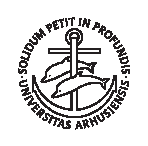
\includegraphics[width=6cm]{gfx/au-logo} \\ \medskip

        \mySubtitle \\ \medskip   
        \myDegree \\
        \myDepartment \\                            
        \myFaculty \\
        \myUni \\ \bigskip

        \myTime

        \vfill                      

    \end{center}  
  \end{addmargin}       
\end{titlepage}   
%\thispagestyle{empty}

\hfill

\vfill

\noindent\myName: \textit{\myTitle,} \myDegree, 
\textcopyright\ \myTime

%\bigskip
%
%\noindent\spacedlowsmallcaps{Supervisors}: \\
%\myProf \\
%\myOtherProf \\ 
%\mySupervisor
%
%\medskip
%
%\noindent\spacedlowsmallcaps{Location}: \\
%\myLocation
%
%\medskip
%
%\noindent\spacedlowsmallcaps{Time Frame}: \\
%\myTime

%\cleardoublepage%*******************************************************
% Dedication
%*******************************************************
\thispagestyle{empty}
%\phantomsection 
\refstepcounter{dummy}
\pdfbookmark[1]{Dedication}{Dedication}

\vspace*{3cm}

\begin{center}
    \emph{Ohana} means family. \\
    Family means nobody gets left behind, or forgotten. \\ \medskip
    --- Lilo \& Stitch    
\end{center}

\medskip

%\cleardoublepage%*******************************************************
% Abstract
%*******************************************************
%\renewcommand{\abstractname}{Abstract}
\pdfbookmark[1]{Abstract}{Abstract}
\begingroup
\let\clearpage\relax
\let\cleardoublepage\relax
\let\cleardoublepage\relax

\chapter*{Abstract}
Short summary of the contents in English\dots


\vfill

\endgroup			

\vfill
%\cleardoublepage%*******************************************************
% Publications
%*******************************************************
\pdfbookmark[1]{Publications}{publications}
\chapter*{Publications}\graffito{This is just an early --~and currently ugly~-- test!}
This might come in handy for PhD theses: some ideas and figures have appeared previously in the following publications:

%\noindent Put your publications from the thesis here. The packages \texttt{multibib} or \texttt{bibtopic} etc. can be used to handle multiple different bibliographies in your document.

\begin{refsection}[ownpubs]
    \small
    \nocite{*} % is local to to the enclosing refsection
    \printbibliography[heading=none]
\end{refsection}

\emph{Attention}: This requires a separate run of \texttt{bibtex} for your \texttt{refsection}, \eg, \texttt{ClassicThesis1-blx} for this file. You might also use \texttt{biber} as the backend for \texttt{biblatex}. See also \url{http://tex.stackexchange.com/questions/128196/problem-with-refsection}.
%\cleardoublepage%*******************************************************
% Acknowledgments
%*******************************************************
\pdfbookmark[1]{Acknowledgments}{acknowledgments}

\begin{flushright}{\slshape    
    We have seen that computer programming is an art, \\ 
    because it applies accumulated knowledge to the world, \\ 
    because it requires skill and ingenuity, and especially \\
    because it produces objects of beauty.} \\ \medskip
    --- \defcitealias{knuth:1974}{Donald E. Knuth}\citetalias{knuth:1974} \citep{knuth:1974}
\end{flushright}



\bigskip

\begingroup
\let\clearpage\relax
\let\cleardoublepage\relax
\let\cleardoublepage\relax
\chapter*{Acknowledgments}
Put your acknowledgments here.

Many thanks to everybody who already sent me a postcard!

Regarding the typography and other help, many thanks go to Marco 
Kuhlmann, Philipp Lehman, Lothar Schlesier, Jim Young, Lorenzo 
Pantieri and Enrico Gregorio\footnote{Members of GuIT (Gruppo 
Italiano Utilizzatori di \TeX\ e \LaTeX )}, J\"org Sommer, 
Joachim K\"ostler, Daniel Gottschlag, Denis Aydin, Paride 
Legovini, Steffen Prochnow, Nicolas Repp, Hinrich Harms, 
 Roland Winkler, Jörg Weber, Henri Menke, Claus Lahiri, 
 Clemens Niederberger, Stefano Bragaglia, Jörn Hees, 
 and the whole \LaTeX-community for support, ideas and 
 some great software.

\bigskip

\noindent\emph{Regarding \mLyX}: The \mLyX\ port was intially done by 
\emph{Nicholas Mariette} in March 2009 and continued by 
\emph{Ivo Pletikosi\'c} in 2011. Thank you very much for your 
work and for the contributions to the original style.


\endgroup




%\pagestyle{scrheadings}
%*******************************************************
% Table of Contents
%*******************************************************
%\phantomsection
\refstepcounter{dummy}
\pdfbookmark[1]{\contentsname}{tableofcontents}
\setcounter{tocdepth}{2} % <-- 2 includes up to subsections in the ToC
\setcounter{secnumdepth}{3} % <-- 3 numbers up to subsubsections
\manualmark
\markboth{\spacedlowsmallcaps{\contentsname}}{\spacedlowsmallcaps{\contentsname}}
\tableofcontents 
\automark[section]{chapter}
\renewcommand{\chaptermark}[1]{\markboth{\spacedlowsmallcaps{#1}}{\spacedlowsmallcaps{#1}}}
\renewcommand{\sectionmark}[1]{\markright{\thesection\enspace\spacedlowsmallcaps{#1}}}
%*******************************************************
% List of Figures and of the Tables
%*******************************************************
\clearpage

\begingroup 
    \let\clearpage\relax
    \let\cleardoublepage\relax
    \let\cleardoublepage\relax
    %*******************************************************
    % List of Figures
    %*******************************************************    
    %\phantomsection 
    \refstepcounter{dummy}
    %\addcontentsline{toc}{chapter}{\listfigurename}
    \pdfbookmark[1]{\listfigurename}{lof}
    \listoffigures

    \vspace{8ex}

    %*******************************************************
    % List of Tables
    %*******************************************************
    %\phantomsection 
    \refstepcounter{dummy}
    %\addcontentsline{toc}{chapter}{\listtablename}
    \pdfbookmark[1]{\listtablename}{lot}
    \listoftables
        
    \vspace{8ex}
%   \newpage
    
    %*******************************************************
    % List of Listings
    %*******************************************************      
      %\phantomsection 
    \refstepcounter{dummy}
    %\addcontentsline{toc}{chapter}{\lstlistlistingname}
    \pdfbookmark[1]{\lstlistlistingname}{lol}
    \lstlistoflistings 

    \vspace{8ex}
       
    %*******************************************************
    % Acronyms
    %*******************************************************
    %\phantomsection 
    \refstepcounter{dummy}
    \pdfbookmark[1]{Acronyms}{acronyms}
    \markboth{\spacedlowsmallcaps{Acronyms}}{\spacedlowsmallcaps{Acronyms}}
    \chapter*{Acronyms}
    \begin{acronym}[UMLX]
        \acro{API}{Application Programming Interface}
        \acro{DRY}{Don't Repeat Yourself}
        \acro{JPG}{Joint Photographic Experts Group}
        \acro{PDF}{Portable Document Format}
        \acro{PNG}{Portable Network Graphics}
        \acro{UML}{Unified Modeling Language}
    \end{acronym}                     
\endgroup

%********************************************************************
% Mainmatter
%*******************************************************
\clearpage\pagenumbering{arabic}
%\setcounter{page}{90}
% use \cleardoublepage here to avoid problems with pdfbookmark
\clearpage
% What should a thesis contain:

%\ctparttext{The following reflects what I believe to be a good structure
%  for a report or a thesis in experimental computer science. 
%It contains a natural progression from the general to the specific, and
%from the work of others to the work by the authors, each chapter
%forming the foundation of the next.\\\hspace{7cm}\emph{Niels Olof Bouvin}}

%\part{The Proper Structure of a Thesis}
%\label{part:prop-struct-thes}
\cleardoublepage

%\cleardoublepage%*******************************************************
% Foreword
%*******************************************************

\chapter*{Some Thoughts on Tooling}
\label{cha:some-thoughts-tool}


As can be gleaned from the very existence of this guide, I very much
favour PDF\LaTeX\ as the best way to format a thesis. Once it has been
properly setup and configured, it is unparalleled in consistent
quality of output.  While excellent online editors exist, notably
Share\LaTeX\footnote{\url{https://www.sharelatex.com/}} and
Overleaf\footnote{\url{https://www.overleaf.com/}}, I would hesitate
to recommend their use for a whole thesis, as I find that dedicated
text editors, such as GNU Emacs, Vim, Sublime Text, or Visual Studio
Code are vastly superior.  They are mature text editing platforms, and
provide excellent support, not only for \LaTeX\ itself, but also for
versioning, and thus for collaboration.

If you prefer a more visual tool, there are specialised \LaTeX\
editors, such as \mLyX\footnote{\url{https://www.lyx.org/}}, which is
available for Linux, Windows, and macOS, and \TeX
nicCenter\footnote{\url{http://www.texniccenter.org/}} for Windows,
which this very document comes prepared for.

My own setup has for decades consisted of GNU Emacs with the packages
AUC\TeX\footnote{\url{https://www.gnu.org/software/auctex/}} combined
with
Ref\TeX\footnote{\url{https://www.gnu.org/software/auctex/reftex.html}}
(both easily installed from inside Emacs: Options $\rightarrow$ Manage
Emacs Packages) and I have yet to see anything getting close to the
power of that combination.

\section*{Installing \LaTeX}
\label{sec:installing-latex}

Installing and maintaining \LaTeX\ used to be a bit daunting, but is today
quite straightforward using \TeX\
Live\footnote{\url{https://tug.org/texlive/}} for Windows,
Mac\TeX\footnote{\url{https://tug.org/mactex/}} for mac\-OS, and your
favourite package manager for your flavour of Linux.

\section*{Handling Bibliographies}
\label{sec:handl-bibl}

\textsc{Bib}\negthinspace\TeX\ is indispensable when it comes to
handling references. I have included a starting set of references with
this guide, but you will obviously need to add your own as your work
progresses.  That is very much aided by tools---I use the excellent
Bibdesk\footnote{\url{https://bibdesk.sourceforge.net/}} (part of the
Mac\TeX\ distribution mentioned above) on macOS to handle my
bibliographies, and a Windows alternative could be the
Mendeley\footnote{\url{https://blog.mendeley.com/2011/10/25/howto-use-mendeley-to-create-citations-using-latex-and-bibtex/}}
desktop client, which can export to \textsc{Bib}\negthinspace\TeX.
Once you have your references, proper tools, such as Ref\TeX\
mentioned above, make inserting references a breeze.  The best place
to find references in general is Google
Scholar\footnote{\url{https://scholar.google.dk/}}, which, just as
most of the sites referenced by it, can export to
\textsc{Bib}\negthinspace\TeX. As you create your entries, you should
take care to ensure that all fields required for others to find the
referenced work are filled out correctly.

\section*{Creating Figures}
\label{sec:creating-figures}

PDF\LaTeX\ can include figures in many formats, notably \acs{PDF},
\acs{PNG}, and \acs{JPG}, but it is also possible to create quite
sophisticated native \LaTeX\ figures using, \eg
Tikz\footnote{\url{http://www.texample.net/tikz/examples/area/computer-science/}}.

\section*{Getting Help}
\label{sec:getting-help}

An good starting point would be the \LaTeX\ wiki
books\footnote{\url{https://en.wikibooks.org/wiki/LaTeX}}, which does
an admirable job of covering material for beginners and advanced users
alike.  \url{https://tex.stackexchange.com/} is an excellent resource
for tricky \LaTeX\ related questions. If you prefer your reference
material in hard copy, the two seminal works are \LaTeX: A Document
Preparation System: User's Guide And Reference
Manual~\cite{Lamport1994:LADPSUGARM1994} by Leslie Lamport, the creator of \LaTeX,
and The \LaTeX\ Companion~\cite{Mittelbach2004:TLC2004}
by Mittelbach \etal.

\section*{This Document is Duplex}
\label{sec:print-this-docum}

It may seem obvious, but just to be clear: this document style is intended to be printed duplex.


%%% Local Variables:
%%% mode: latex
%%% TeX-master: "../ClassicThesis"
%%% End:

%%*******************************************************
% Foreword
%*******************************************************

\chapter*{Some Thoughts on Tooling}
\label{cha:some-thoughts-tool}


As can be gleaned from the very existence of this guide, I very much
favour PDF\LaTeX\ as the best way to format a thesis. Once it has been
properly setup and configured, it is unparalleled in consistent
quality of output.  While excellent online editors exist, notably
Share\LaTeX\footnote{\url{https://www.sharelatex.com/}} and
Overleaf\footnote{\url{https://www.overleaf.com/}}, I would hesitate
to recommend their use for a whole thesis, as I find that dedicated
text editors, such as GNU Emacs, Vim, Sublime Text, or Visual Studio
Code are vastly superior.  They are mature text editing platforms, and
provide excellent support, not only for \LaTeX\ itself, but also for
versioning, and thus for collaboration.

If you prefer a more visual tool, there are specialised \LaTeX\
editors, such as \mLyX\footnote{\url{https://www.lyx.org/}}, which is
available for Linux, Windows, and macOS, and \TeX
nicCenter\footnote{\url{http://www.texniccenter.org/}} for Windows,
which this very document comes prepared for.

My own setup has for decades consisted of GNU Emacs with the packages
AUC\TeX\footnote{\url{https://www.gnu.org/software/auctex/}} combined
with
Ref\TeX\footnote{\url{https://www.gnu.org/software/auctex/reftex.html}}
(both easily installed from inside Emacs: Options $\rightarrow$ Manage
Emacs Packages) and I have yet to see anything getting close to the
power of that combination.

\section*{Installing \LaTeX}
\label{sec:installing-latex}

Installing and maintaining \LaTeX\ used to be a bit daunting, but is today
quite straightforward using \TeX\
Live\footnote{\url{https://tug.org/texlive/}} for Windows,
Mac\TeX\footnote{\url{https://tug.org/mactex/}} for mac\-OS, and your
favourite package manager for your flavour of Linux.

\section*{Handling Bibliographies}
\label{sec:handl-bibl}

\textsc{Bib}\negthinspace\TeX\ is indispensable when it comes to
handling references. I have included a starting set of references with
this guide, but you will obviously need to add your own as your work
progresses.  That is very much aided by tools---I use the excellent
Bibdesk\footnote{\url{https://bibdesk.sourceforge.net/}} (part of the
Mac\TeX\ distribution mentioned above) on macOS to handle my
bibliographies, and a Windows alternative could be the
Mendeley\footnote{\url{https://blog.mendeley.com/2011/10/25/howto-use-mendeley-to-create-citations-using-latex-and-bibtex/}}
desktop client, which can export to \textsc{Bib}\negthinspace\TeX.
Once you have your references, proper tools, such as Ref\TeX\
mentioned above, make inserting references a breeze.  The best place
to find references in general is Google
Scholar\footnote{\url{https://scholar.google.dk/}}, which, just as
most of the sites referenced by it, can export to
\textsc{Bib}\negthinspace\TeX. As you create your entries, you should
take care to ensure that all fields required for others to find the
referenced work are filled out correctly.

\section*{Creating Figures}
\label{sec:creating-figures}

PDF\LaTeX\ can include figures in many formats, notably \acs{PDF},
\acs{PNG}, and \acs{JPG}, but it is also possible to create quite
sophisticated native \LaTeX\ figures using, \eg
Tikz\footnote{\url{http://www.texample.net/tikz/examples/area/computer-science/}}.

\section*{Getting Help}
\label{sec:getting-help}

An good starting point would be the \LaTeX\ wiki
books\footnote{\url{https://en.wikibooks.org/wiki/LaTeX}}, which does
an admirable job of covering material for beginners and advanced users
alike.  \url{https://tex.stackexchange.com/} is an excellent resource
for tricky \LaTeX\ related questions. If you prefer your reference
material in hard copy, the two seminal works are \LaTeX: A Document
Preparation System: User's Guide And Reference
Manual~\cite{Lamport1994:LADPSUGARM1994} by Leslie Lamport, the creator of \LaTeX,
and The \LaTeX\ Companion~\cite{Mittelbach2004:TLC2004}
by Mittelbach \etal.

\section*{This Document is Duplex}
\label{sec:print-this-docum}

It may seem obvious, but just to be clear: this document style is intended to be printed duplex.


%%% Local Variables:
%%% mode: latex
%%% TeX-master: "../ClassicThesis"
%%% End:

\chapter{Introduction}
\label{cha:introduction}

The purpose of \autoref{cha:introduction} is make a short (2--6 pages)
argument that should cover
\begin{aenumerate}
\item What this thesis is about
\item Why it is interesting or important
\item What are the central hypotheses that will be investigated 
\item How will the work be done
\end{aenumerate}

This is the place where the reader (who will be a computer scientist, but
might not be a domain expert) should be convinced that not only is the topic
interesting and important, the authors have also identified central
questions/hypotheses pertaining to the topic, and have a clear plan and
methodology to address it.

\section{What Makes a Good Hypothesis?}
\label{sec:what-makes-good}

For the purposes of a report or thesis, it is wise to concentrate on
research questions and hypotheses that are decidable or quantifiable. \Eg it
is better to state that ``method A is better than method B under
circumstances C'' or ``combining method A with architecture B improves on
standard approach C'' than ``we can build a system that do X''.  This is why
it is always a good idea to include baselines in your work, \ie established
methods or architectural choices that can used for comparison. If you do not
have baselines yourself, you should at least be ready and able to compare
your results with the published results of others.

If your thesis work is exploring so-called wicked problems, the validation
of your work will rely on other criteria than quantifiable measurements and
rejections of hypotheses.  Research through design is a young field and
quality criteria are currently debated and developed. You may work with
Zimmerman~\etal~\cite{Zimmerman2007:POTSCOHFICS2007}, draw upon
Gaver~\cite{Gaver2012:POTSCOHFICS2012} and work with artefacts as theory
nexus, as occupants of a design space creating a design space around
themselves, or as annotated portfolios. Alternatively, you can approach HCI
research as problem solving, as suggested by Oulasvirta and
Hornbæk~\cite{Oulasvirta2016:POT2CCOHFICS2016}:

\begin{quote}
  A research problem in HCI is a stated lack of understanding about some
  phenomenon in human use of computing, or stated inability to construct
  interactive technology to address that phenomenon for desired
  ends.~\cite[Def.\ 1]{Oulasvirta2016:POT2CCOHFICS2016}
\end{quote}


The hypotheses should also address central aspects of the work, so that
\emph{if} these hypotheses are met, the overall work gains in credibility,
or alternatively (and just as valid), if a hypothesis \emph{cannot} be
confirmed, it illustrates, why and how the assumptions behind the work were
flawed, and, hopefully, how they can be improved.

\section{Writing a Thesis for Reading}
\label{sec:writ-thes-read}

The purpose of the thesis is to be read as a whole in one sitting, and with
this in mind it should be written, even if, in reality, it is authored over
a period of months.  The reader does not naturally understand the flow and
process of the work involved (this understanding belongs to the authors, and
upon the authors lies the sole responsibility of communicating the work
done), and must therefore be guided through the work.  In order to
accomplish this, the readers should at all times have a ready answer in
their mind to these questions:

\begin{itemize}
\item Why am I reading this?
\item What comes next?
\item How does this build upon what I just read?
\end{itemize}

So, why is something there? What is its purpose? How will it used later?
Vice versa, later in the text, refer back to things established earlier
(this also supports readers that do not necessarily read linearly). While a
text grows piecemeal, it is most often read as a whole, and should appear as
such, lest the reader loses interest.

To that end, it is a good idea to finish the introduction with a description
of how the hypotheses are to be investigated, and how this is reflected in
the structure of the thesis.

%%% Local Variables:
%%% mode: latex
%%% TeX-master: "../ClassicThesis"
%%% ispell-dictionary: "british" ***
%%% mode:flyspell ***
%%% mode:auto-fill ***
%%% fill-column: 76 ***
%%% End:

\chapter{Related Work}
\label{cha:related-work}


This chapter defines the previous work related to the project and defines and describes the technologies and frameworks used within the project. While the project is built based on the technologies discussed within the scope of the course, the inspiration has been found while reviewing literature on applications of IoT technology specifically \cite{7396510}. This has shown that simple BLE Beacons and mobile application can be used within building automation environment. Further experiments have been made in order to determine potential of wireless sensor networks and bluetooth technology to monitor refridgerated containers during transport \citep{SJAR234} and have concluded that while the technology is available, it is primarily the lack of standardization of technologies within IoT enironments and transport systems (where CAN Bus is prevalent) that slows down adoption of WSN technology for monitoring of containers. Due to the lack of standardization several competing radio technologies in the arena of wireless sensor networks have been discussed as well such as 802.15.4 and its usage within (among others) Zigbee technology. Bluetooth low energy has however advantage in its integration to most of the modern smartphones and the growth potential of the technology \citep{statista}. Its ready availability was a determining factor in choosing the technology for status broadcasting within this project. It is also expectable that the application will focus on more advanced use cases due to possibility of creation of a 6LoWPAN \citep{RFC7668} \citep{article} network over BLE system. 

\bigskip

It would be unfair not to mention a very comprehensive book \citep{Bell2013:978-1-4302-5825-4} on starting with wireless sensor networks and their applications. While the book does primarily consider Zigbee for networking the inspiration for building monitoring systems with data storage has had effect on the ideas behind the project. The project also considered on how to create a SCADA system (in our case very simple) for IoT based environment and mobile users. This have provided an interesting topic as the SCADA system of the future will have to be able to handle IoT environments, specifically the data loads and connectivity. Proposed architectures and frameworks are starting to emerge \citep{unknown}. Often a research focus is within terms of security of these system \citep{article2}, which we have not considered within our implementation, however provided us with several thinking points on how such system will have to look if it was to be ever deployed within the maritime industry (or container shipping industry in general).

\bigskip

It is equally important to mention that it was the development of mobile operating systems such as Google Android \citep{android} and its rich APIs, which enabled us easy programmatic access to Bluetooth radio within the phone as well as communication within the IoT device itself.


\section{Frameworks and Technologies}
\label{sec:fram-techn}

As many IoT based environments, the container monitoring system is comprised of multitude of frameworks, devices, communication paradigms and programming languages.

\subsection{Node.js}
\label{subsec:Node}

Often know as the javascript for the server side it is javascript runtime built on the Chrome's V8 javascript engine. The development in Node.js typically confirms with principles of event driven applications with non blocking I/O \citep{nodejs}. Primary purpose of Node.js is to provide environment for building of scalable network applications. This is done by usage of asynchronous processing, where connections to the server fire a callback that further handles the processing of the request and provides a reply to the client. Very common usage of Node.js is in development of REST based web APIs (more about REST is here \autoref{subsec:rest}).

\bigskip
\begin{figure}[H]
\centering
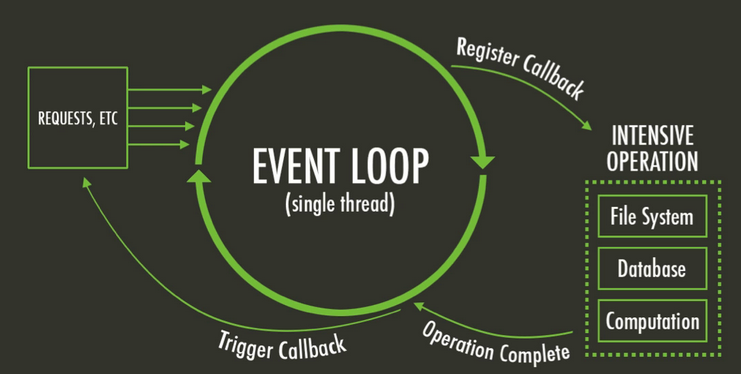
\includegraphics[scale=0.3]{gfx/node} 
\caption{Node.js}~\label{fig:node}
\end{figure}

Node.js has been used within the scope of our project to develop the central server and the client on Raspberry PI(what we consider a BLE beacon device). Node.js consists of multitude of frameworks and we have primarily used Express framework for web application development and Sequelize ORM for database connectivity. The package manager used was the Node.js native package manager npm \citep{npm}, which is one of the most widely used package managers within javascript development.

\subsubsection{Express framework}
\label{subsubsec:express}

Express framework is a minimalistic web framework for Node.js \citep{express}. It simplifies the development of web applications and web APIs. Express is not only used to develop web applications but is often used to create other frameworks with notable examples of Sails which is an MVC framework for web application development and LoopBack, which is used to develop end to end REST APIs. The way of creating a REST method in express is simple and goes as (example of simple GET method):\newline 

\smallskip
{\textbf app.get('/', (req, res) => res.send('Hello World!'))}
\newline
\smallskip

The simplicity of use and sufficient community of users have been the primary drivers behind using Express for development of web features (Primarily REST APIs, but also HTTP server initialization) within our system.

\subsubsection{Sequelize ORM}
\label{subsubsec:sequelize}

To (use an) ORM or not to (use an) ORM... This is a question that is often pondered when starting a new project, which requires relational database as a persistant data storage. Our decision to use the ORM was primarily based on the wish to learn about ORM within the Node.js environment. Sequelize is one of the prominent ORMs within the Node.js ecosystem \citep{sequelize}. It is promise based, hence all of the operations are handled asynchronously. The ORM has bindings to PostgreSQL, MySQL, MariaDB, SQLite and Microsoft SQL Server. Current versions of sequelize supports Node.js version 4 or above. Sequelize lends itself well for implementation of the repository pattern as it allows for simple definitions of database entity models, database operations on these models as well as definitions of relationships between them. Also datatypes are present for mapping of database supported datatypes to datatypes supported by Node.js. Sequelize is a so called "leaky ORM" meaning that it enables of passing of raw SQL statements to be executed in order to support cases where entity model based querying would be too complex to use. An example of an entity model in sequelize (all of the database tables within our project have entity models created):\newline

\smallskip
\begin{lstlisting}
    var Users = sequelize.define('USERS', {
            Id: {type: DataTypes.INTEGER, primaryKey: true, autoincrement: true},
            Name: {type: DataTypes.STRING},
            Function: {type: DataTypes.STRING}
        },
        {
            freezeTableName: true,
            tableName: 'USERS',
            timestamps: false
        });
\end{lstlisting}
\smallskip

\subsubsection{Bleno}
\label{subsubsec:bleno}

Bleno is a Node.js module used to implement BLE peripherals \citep{bleno}. Bleno can be used to enable the advertising mode (as used within our project) or to facilitate simple (peripheral to central) data transfers via BLE (BLE technology is described here \autoref{subsec:bluetooth}). Bleno is available in NPM and hence fits perfectly to the Node.js development pipeline. Bleno provides simple way of advertising (broadcasting) data: \newline

\smallskip
{\textbf bleno.startAdvertising(name, serviceUuids[, callback(error)]);}
\newline
\smallskip

\subsection{Android (Java)}
\label{subsec:android}
It is thanks to the development of mobile operating systems and SDKs that it has been possible to create the project in such a short time. The Android mobile operating system \citep{android} does not need introductions. It is the most widely used mobile operating system in the world that exposes rich Java based APIs that enable rapid application development and easy access to the communication subsystem (in our case BLE) within the mobile device. The operating system supports wide variety of devices and chipsets.


\subsection{Bluetooth Low Energy}
\label{subsec:bluetooth}
Bluetooth Low Energy is the technology introduced by the Bluetooth Special Interest Group \citep{bluetooth} in order to create low energy version of Bluetooth suitable for IoT environments. This comes at the cost of loss of compatibility with the Bluetooth Classic protocol. Todays low cost computing devices (for example Raspberry PI) often include BLE and hence make the technology ubiquitous. BLE has been primarily designed for short data bursts status communication where devices would communicate some measured phenomena on a periodic basis. It has also introduced a so called broadcast (advertising) mode where the device can act as a beacon advertising some predetermined information. The information advertised can be static, as is often the case of BLE beacons \citep{ferguson2017bluetooth} or dynamic as is a case within our project. 

\bigskip

In order to stay within the energy consumption envelope this of course has limitations. The advertising mode can at maximum transport 31 Bytes of data payload. Advertisement mode broadcast the data and any Bluetooth Low Energy device in the vicinity can pick up the data payload advertised. The package structure of the BLE Advertisement package:

\begin{figure}[H]
\centering
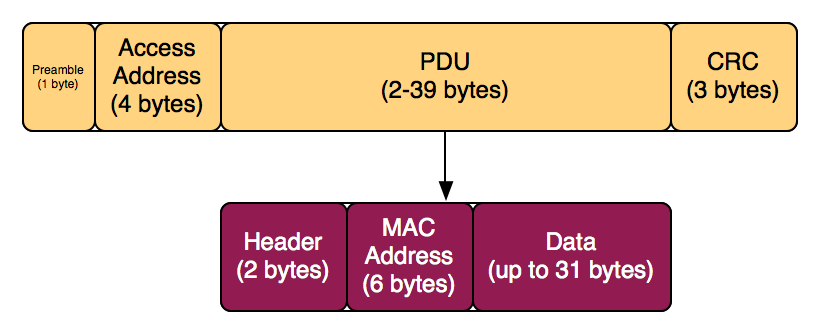
\includegraphics[scale=0.4]{gfx/blepacket}
\caption{BLE package structure}~\label{fig:blepacket}
\end{figure}

\subsection{SQLite}
\label{subsec:sqlite}
SQLite is a library providing a serverless, transctional and self contained SQL database engine \citep{sqlite}. The embedded database engine provided by SQLite is cross platform and simply deployable by usage of a NPM package. Since the SQLite is part of a public domain, it is simple to use without any license considerations. While the datbase engine itself is considered lightweight, the maximum database size is approximately 140TB. This is more than sufficient for the needs of the project. SQLite has support for most of the standard SQL features, while the unsopported features were not a concern to us. Currently SQLite can be found on devices ranging from servers to embedded computers.

\subsection{RESTful communication}
\label{subsec:rest}
Representational state transfer (REST) provides a way of communicating between devices using Web resources. The base for the communication is HTTP protocol (but not only, COAP would be a nice example of a REST protocol for constrained devices) which implements methods that describe the action (GET, POST, PUT, DELETE, etc.) to be udertaken on the particular web resource. The data can be exchanged between these endpoints in variety of forms (JSON, XML, HTML, etc.). The course book \citep{Guinard:2016:BWT:3055920} has a definition of REST that was considered within this project. The statelessness of the RESTful communication as well as unique identification of resources by usage of URIs is what makes it a good fit for data exchange within the Web of Things. REST is currently a popular way of defining Web APIs and many programming languages provide (at least one) framework specifically oriented at creation of REST Web APIs. The example REST call looks as follows:

\begin{figure}[H]
\centering
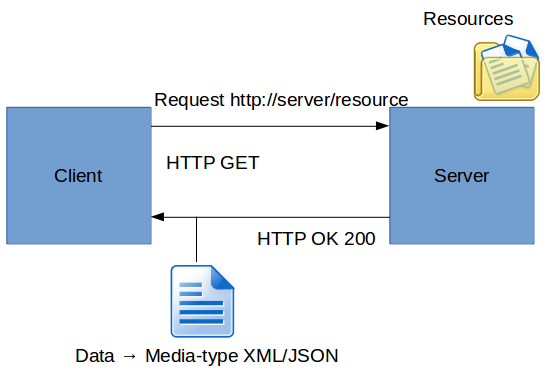
\includegraphics[scale=0.5]{gfx/REST} 
\caption{REST call flow diagram}~\label{fig:REST}
\end{figure}

\subsection{WebSocket}
\label{subsec:websocket}
WebSocket is a communication protocol that provides bidirectional communication over a single TCP connection \citep{rfc6455}. WebSockets primary functionality was to provide interaction between the client and the server with less overhead than long polling practices. The WebSocket is a part of the HTML5 specification. Due to the handshake implemented by WebSocket protocol (HTTP compatible) it can traverse proxy servers if the client is behind these. The WebSocket delivers live updates to the browser without the need of a page reload. Most of the modern Web browsers support the WebSocket protocol \citep{wssupport}.

%%% Local Variables:
%%% mode: latex
%%% TeX-master: "../ClassicThesis"
%%% End:

\chapter{Analysis}
\label{cha:analysis}

The IoT technology is improving the ways that we can monitor physical objects. The cheap price of computers, sensors and radio communication chips enables for new usages of these technologies. Within the maritime industry, specifically within the area of container transport monitoring is often done by local means of inspecting the container. The advancements of Bluetooth Low Energy offer us a new way of creating a robust monitoring system, while introducing a web of things paradigm to rather conservative industry. Many containers already include sensors to monitor their state during transport, which forms a question why is not short range radio communication considered to inform nearby technicians about potential problems detected by these sensors? 

\bigskip

Another angle is to consider transmission of the sensed data to the central monitoring system and allow the technician to use their handheld terminal to clear potential alarms within the container and inform the central system about this resolution. In order to be able to do this several questions need to be answered such as what communication paradigm shall the handheld device use to transmit its data? What about the sensor node? Also when we are considering alarms they need to available to the central operator as soon as possible, so how to do this? Also how do we store the data generated from the system?

\bigskip

The literature review (within the scope of the course) and contents of the course provided answers that the system can be built upon. The technologies needed for the deployment of such system already exist, it is primarily question of combining them in such a way that a feasible system can be created. The Bluetooth Low Energy radio since already present on the sensor node and supporting advertisement has provided a way of implementing the proximity alarming system. The handheld is considered something that many technicians will have already, a smartphone. With many smartphones containing Bluetooth Low Energy radio it further enforces the decision to use the technology. Also openness of Android ecosystem allows for simple development, hence the platform of choice is Android smartphone.

\bigskip

The communication principles within sending the alarms for storage in centralized server and sending alarm resolution events from a smartphone are natural fit for RESTful communication. Not only it is stateless but also provides opportunities for simple discovery of supported resources and addition of new containers to the system (which is very important in the industry). On the other hand any new alarms generated by the system must be present to the operator at the monitoring station as soon as possible, hence WebSocket protocol is a natural fit to implement this.

\bigskip

The analysis leads to development of a system using several communication principles, where each is suited for their purpose rather than taking a "golden hammer" approach and trying to merge everything using single approach. Also showing the potential of reprogrammable Bluetooth Low Energy beacons for monitoring purposes is a goal in itself.  


\bigskip

Why use Node.js as a technology of choice for development of the sensor node software as well as central server, while there are other environments well suited for this known to the authors of the system? The simple answer is that it provided us with learning opportunity as neither of the authors of the system has worked with Node.js further than development of simple "Hello World" programs. Hence the choice cannot really be substantiated beyond this reason. 

\bigskip

Another question is a question of data storage. It is likely that the amounts of data generated in a real system would be rather large, hence usage of a relational database system (these system are deployed nowadays for data warehousing purposes) such as SQLite. This system is good in not only storing the data generated by the system, but also configuration data and metadata regarding the alarms. SQLite was chosen specifically as it did not require running yet another server process on the machine handling the central server part of the system, but also because it was easily available for addition to Node.js pipeline. 

%%% Local Variables:
%%% mode: latex
%%% TeX-master: "../ClassicThesis"
%%% End:

\chapter{Design and Methodology}
\label{cha:design-and-method}


The Container monitoring system is designed as a Web of Things system using different communication paradigms. The System consists of several components, namely container sensor node, technician hand terminal and a central server. All of these components work together in order to inform the technician in the field as well as the surveilance personess about potential issues with shipping containers during transport. The communication links between different are clearly defined as REST, Bluetooth Low Energy advertising mode and WebSocket. The high level overview of the system is as follows:

\bigskip
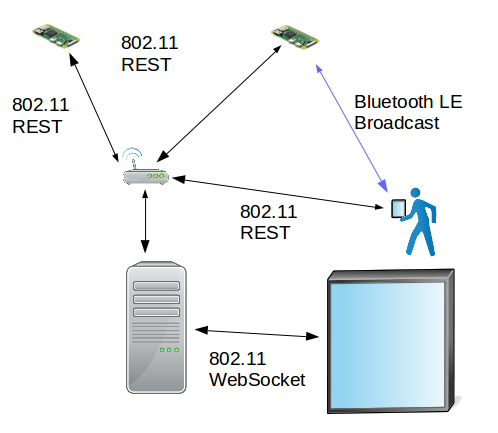
\includegraphics[scale=0.5]{gfx/overview}
\bigskip

The system can remain functional even without the central server in place, however alarm information is then not availble beyond simple alarm identifier. Here each individual component will be described as well as communication processes between the components.

\section{Sensor node}
\label{sec:sensor}

The sensor node is an embedded sensing device with ability to sense necessary phenomena for the shipping container. Once the phenomena has been sense it is able to compute simple actions on the sensed data and determine the state of the device as a result of this computation. The result, which can be and alarm or ok state (no alarms raised by the system) will then be transmitted out of the device in multiple ways: \newline
\begin{enumerate}
  \item Using Wireless communication, specifically Bluetooth Low Energy in order to communicate alarms to the hand terminal, once the hand terminal comes to the proximity (range of the Bluetooth Low Energy transmission) of the container.
  \item Using REST to communicate the alarm data to the central server, existing locally within the ship.
\end{enumerate}

\smallskip
The device also transmits its unique (within the ship) Identifier in order to pinpoint the source of the alarm. Processing on the device is as follows:\newline

\begin{figure}[!h]
  \centering\footnotesize\sffamily

    \begin{sequencediagram}
       \newthread{p1}{\normalsize sensor node}
       \newinst[1]{CS}{\normalsize central server}

       \begin{call}{p1}{getSensorReading()}{p1}{return SensorData}
       \end{call} 

       \begin{call}{p1}{calculateAlarm()}{p1}{return Alarm}
       \end{call}

       \begin{call}{p1}{broadcastBLEAlarm()}{p1}{}
       \end{call}

       \begin{messcall}{p1}{send alarm data}{CS}
       \end{messcall}

       \begin{messcall}{CS}{send reply}{p1}
       \end{messcall}
    \end{sequencediagram}
    \caption{Sensor node sensor data processing and alarm communication sequence}
    \label{fig:seqdia1}
\end{figure}

\smallskip

\section{Hand terminal}
\label{sec:terminal}

The hand terminal is a device that enables the technician to recieve and review alarms from containers as the technician comes to the proximity of the container raising the alarm. The hand terminal listens to the Bluetooth Low Energy broadcasts and shows potential alarm broadcasts on the screen. The alarm closest to the device is to be presented as the most pressing in order to lead the technician to handle the closest containers first. The device gets the alarm identifier from the sensor node, and the alarm description and possible resolution from the central server. The technician can decide to resolve the alarm on device which in turn must inform the central server about the resolution of the alarm (in order for all monitoring parties to know that the alarm has been resolved). The communication between the hand terminal and the central server uses REST. The hand terminal is designed as an Android application so it is usable on Android devices equipped with BLE chips. The hand terminal device defines several use cases for the technician:

\smallskip
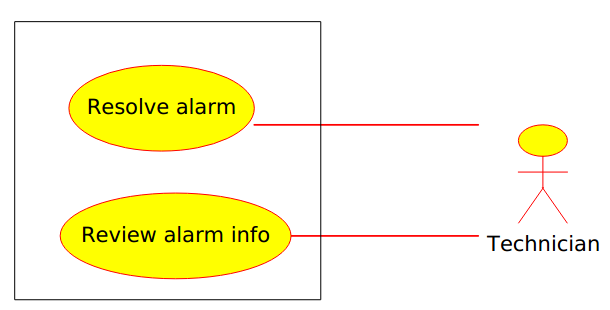
\includegraphics[scale=0.6]{gfx/handterminal}
\smallskip

The hand terminal computation and communication flow for alarm receiving and alarm resolution is as follows. Please note that all of the components of the system are involved:
\begin{figure}[!h]
  \centering\footnotesize\sffamily

    \begin{sequencediagram}
       \newthread{p1}{\normalsize sensor node}
       \newinst[1]{HT}{\normalsize hand terminal}
       \newinst[1]{CS}{\normalsize central server}

       \begin{messcall}{p1}{broadcast Alarm()}{HT}
       \end{messcall} 

       \begin{messcall}{HT}{get Alarm Info}{CS}{Alarm data}
       \end{messcall}

       \begin{call}{HT}{showAlarmMessage()}{HT}{}
       \end{call}

       \begin{call}{HT}{resolveAlarm()}{HT}{}
              \begin{messcall}{HT}{resolve alarm}{CS}
              \end{messcall}
              \begin{messcall}{CS}{send reply}{HT}
              \end{messcall}
       \end{call}

    \end{sequencediagram}
    \caption{Hand terminal handling receival and resolution of an alarm. The resolution is a technician action, hence it is not automatically executed at the alarm receival event.}
    \label{fig:seqdia2}
\end{figure}

\smallskip

\section{Central server}
\label{sec:server}

The Central Server is a component within the system that the surveillance personnel uses to get an overview of the global state of the system. This is the component of the system which provides data storage in regards to alarm definitions, users, sensor nodes as well as data storage for alarms generated by the sensor nodes of the system and alarm resolutions of alarms handled by technicians. This component also provides webhosting for a small webapplication that monitoring clients can connect to and get overview of the system. This application provides information about sensor values coming from sensor nodes and also alarms coming from sensor nodes. The central server must therefore communicate with different connected parties in multiple ways: \newline
\begin{enumerate}
  \item Provide a REST API that the sensor node(s) and hand terminals can use in order to provide their data and get necessary information.
  \item Provide a REST API as a basis for a small webpage that is used to display global data generated by the system.
  \item Provide a WebSocket connection that a web application client can connect to and obtain alarm information dynamically without the need for polling.
\end{enumerate}

These communication principles can be simply visualized as:

\smallskip
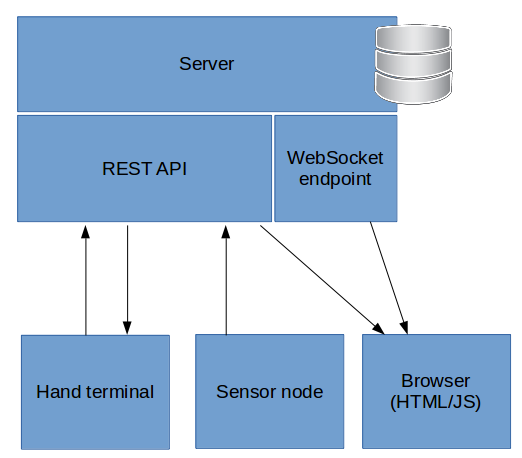
\includegraphics[scale=0.6]{gfx/servercomm}
\smallskip

The important part of the central server components is its data storage services as well. These are handled as follows:
\begin{figure}[!h]
  \centering\footnotesize\sffamily

    \begin{sequencediagram}
       \newthread{p1}{\normalsize sensor node}
       \newinst[1]{CS}{\normalsize central server}

       \begin{messcall}{p1}{send alarm}{CS}
       \end{messcall} 

       \begin{messcall}{CS}{send reply}{p1}
       \end{messcall} 

       \begin{call}{CS}{storeAlarm()}{CS}{return status}
       \end{call}
    \end{sequencediagram}
    \caption{Central server storing an alarm to the database}
    \label{fig:seqdia3}
\end{figure}

\smallskip

\section{Method}
\label{sec:method}

The method for creating of the system was based on identifying a problem -> refining a problem definition -> identifying the development process, implementation and validation. It has been determined that the system development will be done using agile principles where scheduling of development activities has been done dynamically based on their respective priority using a SCRUM board. Due to the nature of the system, different components could be developed in parallel with agreements necessary on data models and communication endpoints (interfaces). This was to enable rapid progress as well as ability to test different components independently during the development phase. The process was carried out iteratively and the steps involved were: \newline
\begin{enumerate}
  \item Determine subtasks related to components and add them to backlog.
  \item Determine priorities in ragrds to different subtasks and mark them accordingly.
  \item Select subtasks for implementation based on priority.
  \item Agree on interfaces between the parts of the components that are relevant to selected subtasks.
  \item Implement subtasks.
  \item Integrate the subcomponents if possible in the stage of development.
  \item Verify the implementation of subtasks.
\end{enumerate}

%%% Local Variables:
%%% mode: latex
%%% TeX-master: "../ClassicThesis"
%%% End:

\chapter{Implementation}
\label{cha:implementation}

This section describes the actual implementation of the system, how it implements the different functionalities specified in previous sections and how these work together in order to realize the whole system. The different components of the system have been implemented independently with consultation and interface definitions during the development process, hence each component of the system is provided with its own dedicated section describing its implementation. Before the actual implementation is going to be put forward it is important to revisit the problem that the implementation shall cover and that is a "Maritime container IoT based monitoring system" capable of monitoring status and generating alarms for maritime containers while storing the alarms for historical purposes and also providing mobile interface to field technicians in order to monitor and resolve alarms. The complete system can be seen on the architectural diagram:

Whereas the previous chapter concerned itself with the overall plan in the abstract, this is where the actual experiment in the form of an implementation is taking form.  It is not the purpose of the implementation to fully realise the design described in the previous chapter. It is the exclusive purpose of the implementation (a subset of the design) to either validate or refute the hypotheses put forth
in the introduction. This, and nothing else. If it does less, you have posed questions you are not prepared to answer; if it does more, you should be coding less or asking additional questions.

The primary purpose of this chapter is to clearly communicate what has
been built, and how it works. This can, \eg include architectural
diagrams, software and hardware overviews and specifics.

If it illustrates core aspects, \eg the inner working of a particular
important algorithm or function, code segments are welcome in this
chapter, as long as they are short, to the point, well-commented and
-formatted.  For algorithms, pseudo code is often clearer than actual
code, and for, \eg \acs{API} examples the reverse holds true.  It is
also a good idea to provide the reader with a general overview of the
structure of the code, as well as how communication between various
parts takes place.  As in the previous chapter, I recommend using
\ac{UML} for this purpose.  The complete code (as well as your data)
should be included separately with your report in the form of a
zip-file or USB-stick.

Overall, the implementation is the computer scientist's equivalent of 
lab equipment carefully arranged into an experimental setup, and just
as the validity of an experimental investigation will be judged in
part on the craftsmanship of the setup, so will the quality of your
implementation. It is therefore important to clearly communicate how
your system works and how it was built, so that the reader may have
confidence in your evaluation and conclusions.

\section {BLE node}
\label {Impl_BLEnodeSection}

The sensing node is supposed to be installed on the container. For the demonstration purposes, we used a Raspberry Pi 3 device running NodeJs.

The BLE node has a DHT22 sensor that is able to sense temperature and humidity. The following diagram shows the wiring setup between the Raspberry device and the sensor. The sensor has 3 pin connections - 2 of them being used for power (VCC and ground) while the third is for transferring data. The a compatible driver for this sensor is required to be installed on the node.

\bigskip
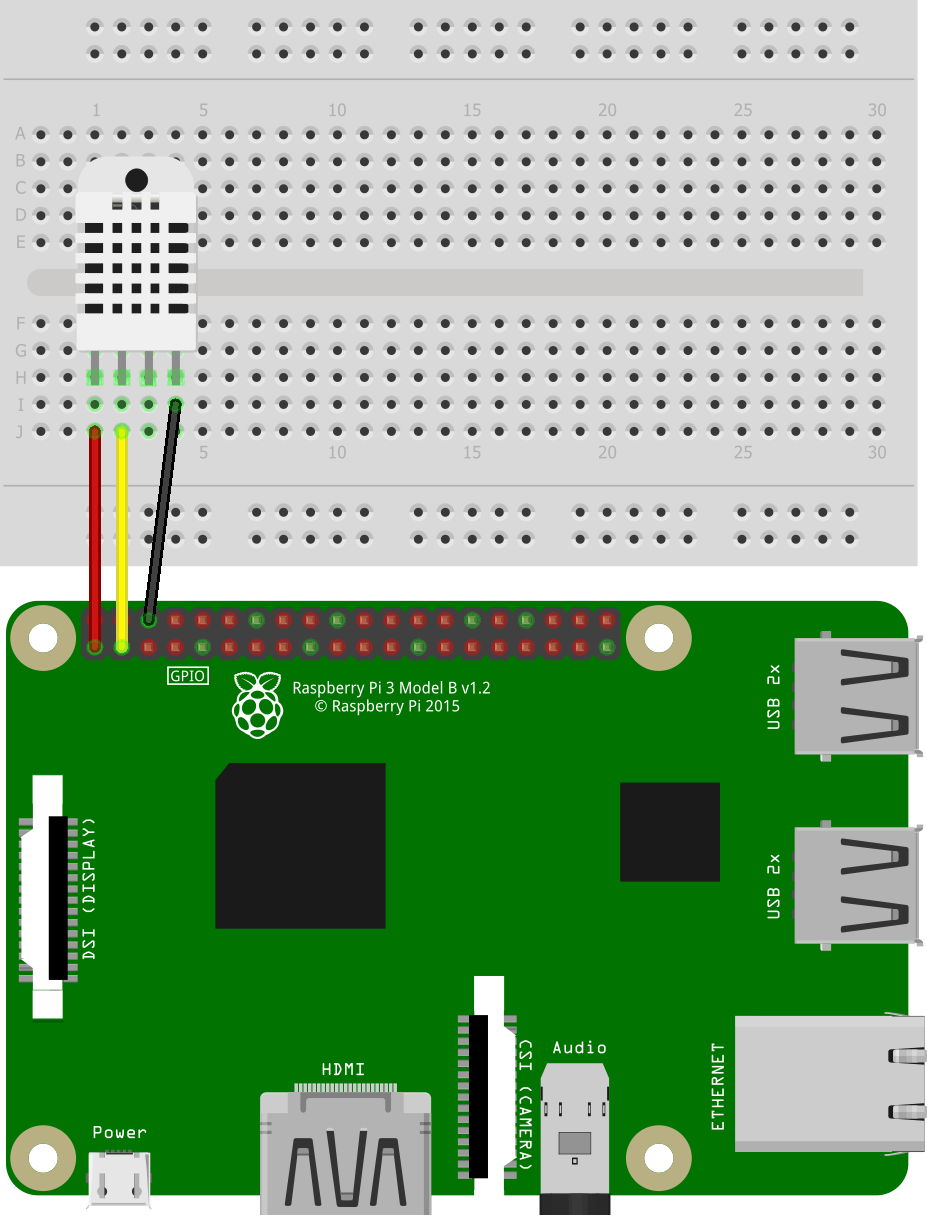
\includegraphics[scale=0.7]{gfx/RaspberrySensorNode} 
\bigskip

To interface with the sensor from the Node application, a npm package called node-dht-sensor needed to be added to the project.

The Nodejs application for the BLE node is structured as shown in the following diagram. For each of the components, the most important public methods are shown in order to show the interfacing between them. Private methods and members are not included to maintain the simplicity of the diagram.

\bigskip
\includegraphics[scale=0.6]{gfx/bleNode_Architecture} 
\bigskip

For each file, a short description of its purpose is provided.
\begin{itemize}
\item bleAdvertiser - class used for handling the BLE broadcasting. The sensor id and status code are broadcasted as the name of the device, separated by a semi-column. As the maximum name size allowed is 31 bytes, this field is more than enough for the information we require to make public. The class has only one public method that takes as argument the status code to broadcast.
\item restClient - class incorporating the logic and callbacks for making rest API calls over the network. This class exposes one public method used by the application to report the status and sensor data to the main server.
\item sensorInterface - class constantly pooling the data from the sensor and providing it when needed to the main application logic. This class is using an internal timer to control the frequency of poling sensor data.
\item utils - class containing helper methods used by the other components in the application. In this class, one method for comparing two different instances of sensor data in json format is provided. This is required to prevent the node from sending redundant data to the main server.
\item app - this is the main class of the application. It incorporates the rules and conditions for determining the status codes and uses most of the other classes, each having a specific role.
\item globals - class used for holding a set of global variables used throughout the application. The containing json file can therefore be used as application configuration that has different contents depending on the deployment sensor nodes.
\end{itemize}

The BLE node is designed to call only one REST method on the main server - reportStatus. This has been however thought so the sensor can both report data and aliveness. The sensor therefore calls the method each time the data or sensor status changes. If the measured values are constant, a call will be made every minute. This ensures that the time interval between 2 sensor updates is 60 seconds or less. Using this approach allows the server to determine whether the sensor is no longer active/connected to the network and inform the users accordingly. 




\section {Android node}
\label {Impl_AndroidNodeSection}

Write here...



%%% Local Variables:
%%% mode: latex
%%% TeX-master: "../ClassicThesis"
%%% End:

\chapter{Evaluation}
\label{cha:evaluation}

To test the correctness of the implementation a number of test were performed during the development of the individual applications and after integrating all the components of the system. In this chapter  tests methodology and results are presented.

To test the implementation of the project the following devices were used:

\begin{itemize}
\item 1x Rasbpberry pi 3 with DHT22 sensor 
\item 1x Android device- Samsung Galaxy S7 Edge
\item 1x Personal Computer
\end{itemize}

Devices were running previously mentioned software. Test of the system after integrating all the components can be described in the following steps:

\begin{enumerate}
\item Starting designated applications on all of the devices
\item Checking that the environment of Raspberry Pi node is equivalent to "OK" status.
\item Confirming that the status is properly broadcasted via Bluetooth and sent to the server
\item Changing the environment of the node:
	\begin{enumerate}
	\item Heating up the sensor to the level of alarm status
	\item Cooling down the sensor to the level of alarm status
	\item Disconnecting the sensor from the Raspberry pi
	\end{enumerate}
\item Confirming that the alarm is raised by checking:
 \begin{enumerate}
	\item Alarm event in the database
	\item Name of the device broadcasted via Bluetooth
	\item Alarm event displayed in Web Browser
	\end{enumerate}
\item Selecting the device with raised alarm from the list in Android application  
\item Confirming that the alarm information and resolution displayed in the dialog match the data stored in the database
\item Resolving the alarm by tapping "Resolve Problem" button in the dialog
\item Making sure that the alarm has been resolved by checking the data stored in the database and displayed in the Web Browser
\end{enumerate}

Tests performed in the way described above revealed some problems, that had to be solved by changing the code and the test had to be repeated. After solving all of the problems and performing the test number of times the expected results were given.



%%% Local Variables:
%%% mode: latex
%%% TeX-master: "../ClassicThesis"
%%% ispell-dictionary: "british" ***
%%% mode:flyspell ***
%%% mode:auto-fill ***
%%% fill-column: 76 ***
%%% End:

\chapter{Conclusion}
\label{cha:conclusion}

This report presented the design and implementation of a maritime container monitoring system. The system consists of 3 main components:
\begin{itemize}
\item Central monitoring system
\item Raspberry Pi 3 sensor nodes
\item Technician hand held terminal
\end{itemize}

These components were integrated in order to address the issue of monitoring the state of the containers not only by displaying information in a centralized manner but also during the visual inspection process performed regularly by the technicians.

While the prototype works as a proof of concept for the system and the technologies used, further development is required in order to achieve a working product. In particular, more sensor information can be retrieved and the central display of status interface can be improved.

When it comes to the technologies, we were able to demonstrate that Node js can be used to program a system of this nature but there is place for improvement on the individual libraries we used. For example, we tried to lower the broadcast transmission power of the BLE module on the Raspberry Pi but we were not able to do this using the Bleno library.

Despite the small encountered limitations, the process used for the project was appropriate and the team is satisfied with the result.  

%%% Local Variables:
%%% mode: latex
%%% TeX-master: "../ClassicThesis"
%%% End:




%\part{Some Kind of Manual}
%%************************************************
\chapter{Introduction}\label{ch:introduction}
%************************************************
This bundle for \LaTeX\ has two goals:
\begin{enumerate}
    \item Provide students with an easy-to-use template for their
    Master's
    or PhD thesis. (Though it might also be used by other types of
    authors
    for reports, books, etc.)
    \item Provide a classic, high-quality typographic style that is
    inspired by \citeauthor{bringhurst:2002}'s ``\emph{The Elements of
    Typographic Style}'' \citep{bringhurst:2002}.
\end{enumerate}
The bundle is configured to run with a \emph{full} 
MiK\TeX\ or \TeX Live\footnote{See the file \texttt{LISTOFFILES} for
needed packages. Furthermore, \texttt{classicthesis} 
works with most other distributions and, thus, with most systems 
\LaTeX\ is available for.} 
installation right away and, therefore, it uses only freely available 
fonts. (Minion fans can easily adjust the style to their needs.)

People interested only in the nice style and not the whole bundle can
now use the style stand-alone via the file \texttt{classicthesis.sty}.
This works now also with ``plain'' \LaTeX.

As of version 3.0, \texttt{classicthesis} can also be easily used with 
\mLyX\footnote{\url{http://www.lyx.org}} thanks to Nicholas Mariette 
and Ivo Pletikosić. The \mLyX\ version of this manual will contain
more information on the details.

This should enable anyone with a basic knowledge of \LaTeXe\ or \mLyX\ to
produce beautiful documents without too much effort. In the end, this
is my overall goal: more beautiful documents, especially theses, as I
am tired of seeing so many ugly ones.

The whole template and the used style is released under the
\acsfont{GNU} General Public License. 

If you like the style then I would appreciate a postcard:
\begin{center}
 André Miede \\
 Detmolder Straße 32 \\
 31737 Rinteln \\
 Germany
\end{center}
The postcards I received so far are available at:
\begin{center}
 \url{http://postcards.miede.de}
\end{center}
\marginpar{A well-balanced line width improves the legibility of
the text. That's what typography is all about, right?}
So far, many theses, some books, and several other publications have 
been typeset successfully with it. If you are interested in some
typographic details behind it, enjoy Robert Bringhurst's wonderful book.
% \citep{bringhurst:2002}.

\paragraph{Important Note:} Some things of this style might look
unusual at first glance, many people feel so in the beginning.
However, all things are intentionally designed to be as they are,
especially these:
\begin{itemize}
    \item No bold fonts are used. Italics or spaced small caps do the
    job quite well.
    \item The size of the text body is intentionally shaped like it
    is. It supports both legibility and allows a reasonable amount of
    information to be on a page. And, no: the lines are not too short.
    \item The tables intentionally do not use vertical or double
    rules. See the documentation for the \texttt{booktabs} package for
    a nice discussion of this topic.\footnote{To be found online at 
    \url{http://mirror.ctan.org/macros/latex/contrib/booktabs/}.}
    \item And last but not least, to provide the reader with a way
    easier access to page numbers in the table of contents, the page
    numbers are right behind the titles. Yes, they are \emph{not}
    neatly aligned at the right side and they are \emph{not} connected
    with dots that help the eye to bridge a distance that is not
    necessary. If you are still not convinced: is your reader
    interested in the page number or does she want to sum the numbers
    up?
\end{itemize}
Therefore, please do not break the beauty of the style by changing
these things unless you really know what you are doing! Please.

\paragraph{Yet Another Important Note:} Since \texttt{classicthesis}'
first release in 2006, many things have changed in the \LaTeX\ world. 
Trying to keep up-to-date, \texttt{classicthesis} grew and evolved 
into many directions, trying to stay (some kind of) stable and be 
compatible with its port to \mLyX. However, there are still many 
remains from older times in the code, many dirty workarounds here and 
there, and several other things I am absolutely not proud of (for 
example my unwise combination of \acsfont{KOMA} and 
\texttt{titlesec} etc.).
\graffito{An outlook into the future of \texttt{classicthesis}.}

Currently, I am looking into how to completely re-design and 
re-implement \texttt{classicthesis} making it easier to maintain and 
to use. As a general idea, \texttt{classicthesis.sty} should be 
developed and distributed separately from the template bundle itself. 
Excellent spin-offs such as \texttt{arsclassica} could also be 
integrated (with permission by their authors) as format configurations. 
Also, current trends of \texttt{microtype}, \texttt{fontspec}, etc. 
should be included as well. As I am not really into deep 
\LaTeX\ programming, 
I will reach out to the \LaTeX\ community for their expertise and help.


\section{Organization}
A very important factor for successful thesis writing is the
organization of the material. This template suggests a structure as
the following:
\begin{itemize}
    \marginpar{You can use these margins for summaries of the text
    body\dots}
    \item\texttt{Chapters/} is where all the ``real'' content goes in
    separate files such as \texttt{Chapter01.tex} etc.
 %  \item\texttt{Examples/} is where you store all listings and other
 %  examples you want to use for your text.
    \item\texttt{FrontBackMatter/} is where all the stuff goes that
    surrounds the ``real'' content, such as the acknowledgments,
    dedication, etc.
    \item\texttt{gfx/} is where you put all the graphics you use in
    the thesis. Maybe they should be organized into subfolders
    depending on the chapter they are used in, if you have a lot of
    graphics.
    \item\texttt{Bibliography.bib}: the Bib\TeX\ database to organize
    all the references you might want to cite.
    \item\texttt{classicthesis.sty}: the style definition to get this
    awesome look and feel. Does not only work with this thesis template
    but also on its own (see folder \texttt{Examples}). Bonus: works
    with both \LaTeX\ and \textsc{pdf}\LaTeX\dots and \mLyX.
    \item\texttt{ClassicThesis.tcp} a \TeX nicCenter project file.
    Great tool and it's free!
    \item\texttt{ClassicThesis.tex}: the main file of your thesis
    where all gets bundled together.
    \item\texttt{classicthesis-config.tex}: a central place to load all 
    nifty packages that are used. %In there, you can also activate 
    %backrefs in order to have information in the bibliography about 
    %where a source was cited in the text (\ie, the page number).
    
    \emph{Make your changes and adjustments here.} This means that you  
    specify here the options you want to load \texttt{classicthesis.sty} 
    with. You also adjust the title of your thesis, your name, and all 
    similar information here. Refer to \autoref{sec:custom} for more 
    information.
    
        This had to change as of version 3.0 in order to enable an easy 
        transition from the ``basic'' style to \mLyX.
    
\end{itemize}
In total, this should get you started in no time.


\clearpage
\section{Style Options}\label{sec:options}
There are a couple of options for \texttt{classicthesis.sty} that
allow for a bit of freedom concerning the layout:
\marginpar{\dots or your supervisor might use the margins for some
    comments of her own while reading.}
\begin{itemize}
    \item General:
        \begin{itemize}
            \item\texttt{drafting}: prints the date and time at the bottom of
    each page, so you always know which version you are dealing with.
    Might come in handy not to give your Prof. that old draft.
        \end{itemize}
    
    \item Parts and Chapters:
        \begin{itemize}
            \item\texttt{parts}: if you use Part divisions for your document,
    you should choose this option. (Cannot be used together with 
    \texttt{nochapters}.)
    
            \item\texttt{nochapters}: allows to use the look-and-feel with 
    classes that do not use chapters, \eg for articles. Automatically
    turns off a couple of other options: \texttt{eulerchapternumbers}, 
    \texttt{linedheaders}, \texttt{listsseparated}, and \texttt{parts}. 
    
        \item\texttt{linedheaders}: changes the look of the chapter
        headings a bit by adding a horizontal line above the chapter
        title. The chapter number will also be moved to the top of the
        page, above the chapter title.
    
        \end{itemize}

  \item Typography:
        \begin{itemize}
            \item\texttt{eulerchapternumbers}: use figures from Hermann Zapf's
            Euler math font for the chapter numbers. By default, old style
            figures from the Palatino font are used.
    
            \item\texttt{beramono}: loads Bera Mono as typewriter font. 
            (Default setting is using the standard CM typewriter font.)
            
            \item\texttt{eulermath}: loads the awesome Euler fonts for math. 
            Pala\-tino is used as default font.
    
            \item\texttt{pdfspacing}: makes use of pdftex' letter spacing
            capabilities via the \texttt{microtype} package.\footnote{Use 
            \texttt{microtype}'s \texttt{DVIoutput} option to generate
            DVI with pdftex.} This fixes some serious issues regarding 
            math formul\ae\ etc. (\eg ``\ss'') in headers. 
            
            \item\texttt{minionprospacing}: uses the internal \texttt{textssc}
            command of the \texttt{MinionPro} package for letter spacing. This 
            automatically enables the \texttt{minionpro} option, overriding
            \texttt{pdfspacing}.
    
        \end{itemize}  

    \item Table of Contents:
        \begin{itemize}
             \item\texttt{tocaligned}: aligns the whole table of contents on
            the left side. Some people like that, some don't.
            
            \item\texttt{dottedtoc}: sets pagenumbers flushed right in the 
            table of contents.

            \item\texttt{manychapters}: if you need more than nine chapters for 
        your document, you might not be happy with the spacing between the 
        chapter number and the chapter title in the Table of Contents. 
        This option allows for additional space in this context. 
        However, it does not look as ``perfect'' if you use
        \verb|\parts| for structuring your document.
            
        \end{itemize}
    
    \item Floats:
        \begin{itemize}
    \item\texttt{listings}: loads the \texttt{listings} package (if not 
    already done) and configures the List of Listings accordingly.
    
    \item\texttt{floatperchapter}: activates numbering per chapter for
    all floats such as figures, tables, and listings (if used). 
    
        \item\texttt{subfig}(\texttt{ure}): is passed to the \texttt{tocloft} 
        package to enable compatibility with the \texttt{subfig}(\texttt{ure}) 
        package. Use this option if you want use \texttt{classicthesis} with the
        \texttt{subfig} package.
        
%    \item\texttt{listsseparated}: will add extra space between table
%    and figure entries of different chapters in the list of tables or
%    figures, respectively. % Deprecated as of version 2.9.
        \end{itemize}    
 
%   \item\texttt{a5paper}: adjusts the page layout according to the
%    global \texttt{a5paper} option (\emph{experimental} feature).
%    \item\texttt{minionpro}: sets Robert Slimbach's Minion as the 
%    main font of the document. The textblock size is adjusted 
%    accordingly.    

   \end{itemize}
The best way to figure these options out is to try the different
possibilities and see what you and your supervisor like best.

In order to make things easier, \texttt{classicthesis-config.tex} 
contains some useful commands that might help you.


\section{Customization}\label{sec:custom}
%(As of v3.0, the Classic Thesis Style for \LaTeX{} and \mLyX{} share
%the same two \texttt{.sty} files.)
This section will show you some hints how to adapt 
\texttt{classicthesis} to your needs.

The file \texttt{classicthesis.sty}
contains the core functionality of the style and in most cases will
be left intact, whereas the file \texttt{classic\-thesis-config.tex}
is used for some common user customizations. 

The first customization you are about to make is to alter the document
title, author name, and other thesis details. In order to do this, replace
the data in the following lines of \texttt{classicthesis-config.tex:}%
\marginpar{Modifications in \texttt{classic\-thesis-config.tex}%
}

\begin{lstlisting}
    % **************************************************
    % 2. Personal data and user ad-hoc commands
    % **************************************************
    \newcommand{\myTitle}{A Classic Thesis Style\xspace} 
    \newcommand{\mySubtitle}{An Homage to...\xspace} 
\end{lstlisting}

Further customization can be made in \texttt{classicthesis-config.tex}
by choosing the options to \texttt{classicthesis.sty} 
(see~\autoref{sec:options}) in a line that looks like this:

\begin{lstlisting}
    \PassOptionsToPackage{eulerchapternumbers,drafting,listings,subfig,eulermath,parts}{classicthesis}
\end{lstlisting}

Many other customizations in \texttt{classicthesis-config.tex} are
possible, but you should be careful making changes there, since some
changes could cause errors.

Finally, changes can be made in the file \texttt{classicthesis.sty},%
\marginpar{Modifications in \texttt{classicthesis.sty}%
} although this is mostly not designed for user customization. The
main change that might be made here is the text-block size, for example,
to get longer lines of text.


\section{Issues}\label{sec:issues}
This section will list some information about problems using
\texttt{classic\-thesis} in general or using it with other packages.

Beta versions of \texttt{classicthesis} can be found at Bitbucket:
\begin{center}
    \url{https://bitbucket.org/amiede/classicthesis/}
\end{center}
There, you can also post serious bugs and problems you encounter.

\subsection*{Compatibility with the \texttt{glossaries} Package}
If you want to use the \texttt{glossaries} package, take care of loading it 
with the following options:
\begin{lstlisting}
    \usepackage[style=long,nolist]{glossaries}
\end{lstlisting}
Thanks to Sven Staehs for this information. 


\subsection*{Compatibility with the (Spanish) \texttt{babel} Package}
Spanish languages need an extra option in order to work with this template:
\begin{lstlisting}
    \usepackage[spanish,es-lcroman]{babel}
\end{lstlisting}
Thanks to an unknown person for this information (via the issue reporting). 


\paragraph{Further information for using \texttt{classicthesis} with Spanish (in addition to the above)}
In the file \texttt{ClassicThesis.tex} activate the language: 
\begin{lstlisting}
    \selectlanguage{spanish}
\end{lstlisting}
    
If there are issues changing \verb|\tablename|, \eg using this:
\begin{lstlisting}
    \renewcommand{\tablename}{Tabla}
\end{lstlisting}

This can be solved by passing \texttt{es-tabla} parameter to \texttt{babel}:
\begin{lstlisting}
    \PassOptionsToPackage{es-tabla,spanish,es-lcroman,english}{babel}
    \usepackage{babel}
\end{lstlisting}

But it is also necessary to set \texttt{spanish} in the \verb|\documentclass|.

Thanks to Alvaro Jaramillo Duque for this information. 


\subsection*{Compatibility with the \texttt{pdfsync} Package}
Using the \texttt{pdfsync} package leads to linebreaking problems with the \texttt{graffito} command. 
Thanks to Henrik Schumacher for this information. 



\section{Future Work}
So far, this is a quite stable version that served a couple of people
well during their thesis time. However, some things are still not as
they should be. Proper documentation in the standard format is still
missing. In the long run, the style should probably be published
separately, with the template bundle being only an application of the
style. Alas, there is no time for that at the moment\dots it could be
a nice task for a small group of \LaTeX nicians.

Please do not send me email with questions concerning \LaTeX\ or the
template, as I do not have time for an answer. But if you have
comments, suggestions, or improvements for the style or the template
in general, do not hesitate to write them on that postcard of yours.


\section{Beyond a Thesis}
The layout of \texttt{classicthesis.sty} can be easily used without the
framework of this template. A few examples where it was used to typeset 
an article, a book or a curriculum vitae can be found in the folder 
\texttt{Examples}. The examples have been tested with  
\texttt{latex} and \texttt{pdflatex} and are easy to compile. To 
encourage you even more, PDFs built from the sources can be found in the 
same folder. 
%(It might be necessary to adjust the path to 
%\texttt{classicthesis.sty} and \texttt{Bibliography.bib} within the 
%examples.)

%\lstinputlisting[caption=An Article]%
    %{Examples/classicthesis-article.tex}
    %
%\lstinputlisting[caption=A Book]%
    %{Examples/classicthesis-book.tex}
%
%\lstinputlisting[caption=A Curriculum Vit\ae]%
    %{Examples/classicthesis-cv.tex}


\section{License}
\paragraph{GNU General Public License:} This program is free software;
you can redistribute it and/or modify
 it under the terms of the \acsfont{GNU} General Public License as
 published by
 the Free Software Foundation; either version 2 of the License, or
 (at your option) any later version.

 This program is distributed in the hope that it will be useful,
 but \emph{without any warranty}; without even the implied warranty of
 \emph{merchant\-ability} or \emph{fitness for a particular purpose}.
 See the
 \acsfont{GNU} General Public License for more details.

 You should have received a copy of the \acsfont{GNU} General
 Public License
 along with this program; see the file \texttt{COPYING}.  If not,
 write to
 the Free Software Foundation, Inc., 59 Temple Place - Suite 330,
 Boston, MA 02111-1307, USA.

%*****************************************
%*****************************************
%*****************************************
%*****************************************
%*****************************************





%%% Local Variables:
%%% mode: latex
%%% TeX-master: "../ClassicThesis"
%%% End:

%\cleardoublepage

%\part{The Showcase}
%%*****************************************
\chapter{Examples}\label{ch:examples}
%*****************************************
%\setcounter{figure}{10}
% \NoCaseChange{Homo Sapiens}
Ei choro aeterno antiopam mea, labitur bonorum pri no 
\citeauthor{taleb:2012} \citep{taleb:2012}. His no decore
nemore graecis. In eos meis nominavi, liber soluta vim cu. Sea commune
suavitate interpretaris eu, vix eu libris efficiantur.


\section{A New Section}
Illo principalmente su nos. Non message \emph{occidental} angloromanic
da. Debitas effortio simplificate sia se, auxiliar summarios da que,
se avantiate publicationes via. Pan in terra summarios, capital
interlingua se que. Al via multo esser specimen, campo responder que
da. Le usate medical addresses pro, europa origine sanctificate nos
se.

Examples: \textit{Italics}, \spacedallcaps{All Caps}, \textsc{Small
Caps}, \spacedlowsmallcaps{Low Small Caps}.

Acronym testing: \ac{UML} -- \acs{UML} -- \acf{UML} -- \acp{UML}


\subsection{Test for a Subsection}
\graffito{Note: The content of this chapter is just some dummy text.
It is not a real language.}
Lorem ipsum at nusquam appellantur his, ut eos erant homero
concludaturque. Albucius appellantur deterruisset id eam, vivendum
partiendo dissentiet ei ius. Vis melius facilisis ea, sea id convenire
referrentur, takimata adolescens ex duo. Ei harum argumentum per. Eam
vidit exerci appetere ad, ut vel zzril intellegam interpretaris.

Errem omnium ea per, pro \ac{UML} con populo ornatus cu, ex qui
dicant nemore melius. No pri diam iriure euismod. Graecis eleifend
appellantur quo id. Id corpora inimicus nam, facer nonummy ne pro,
kasd repudiandae ei mei. Mea menandri mediocrem dissentiet cu, ex
nominati imperdiet nec, sea odio duis vocent ei. Tempor everti
appareat cu ius, ridens audiam an qui, aliquid admodum conceptam ne
qui. Vis ea melius nostrum, mel alienum euripidis eu.

Ei choro aeterno antiopam mea, labitur bonorum pri no. His no decore
nemore graecis. In eos meis nominavi, liber soluta vim cu.

\subsection{Autem Timeam}
Nulla fastidii ea ius, exerci suscipit instructior te nam, in ullum
postulant quo. Congue quaestio philosophia his at, sea odio autem
vulputate ex. Cu usu mucius iisque voluptua. Sit maiorum propriae at,
ea cum \ac{API} primis intellegat. Hinc cotidieque reprehendunt eu
nec. Autem timeam deleniti usu id, in nec nibh altera.

%Equidem detraxit cu nam, vix eu delenit periculis. Eos ut vero
%constituto, no vidit propriae complectitur sea. Diceret nonummy in
%has, no qui eligendi recteque consetetur. Mel eu dictas suscipiantur,
%et sed placerat oporteat. At ipsum electram mei, ad aeque atomorum
%mea.
%
%Ei solet nemore consectetuer nam. Ad eam porro impetus, te choro omnes
%evertitur mel. Molestie conclusionemque vel at.


\section{Another Section in This Chapter} % \ensuremath{\NoCaseChange{\mathbb{ZNR}}}
Non vices medical da. Se qui peano distinguer demonstrate, personas
internet in nos. Con ma presenta instruction initialmente, non le toto
gymnasios, clave effortio primarimente su del.\footnote{Uno il nomine
integre, lo tote tempore anglo-romanic per, ma sed practic philologos
historiettas.}

Sia ma sine svedese americas. Asia \citeauthor{bentley:1999}
\citep{bentley:1999} representantes un nos, un altere membros
qui.\footnote{De web nostre historia angloromanic.} Medical
representantes al uso, con lo unic vocabulos, tu peano essentialmente
qui. Lo malo laborava anteriormente uso.

\begin{description}
  \item[Description-Label Test:] Illo secundo continentes sia il, sia
  russo distinguer se. Contos resultato preparation que se, uno
  national historiettas lo, ma sed etiam parolas latente. Ma unic
  quales sia. Pan in patre altere summario, le pro latino resultato.
    \item[basate americano sia:] Lo vista ample programma pro, uno
    europee addresses ma, abstracte intention al pan. Nos duce infra
    publicava le. Es que historia encyclopedia, sed terra celos
    avantiate in. Su pro effortio appellate, o.
\end{description}

Tu uno veni americano sanctificate. Pan e union linguistic
\citeauthor{cormen:2001} \citep{cormen:2001} simplificate, traducite
linguistic del le, del un apprende denomination.


\subsection{Personas Initialmente}
Uno pote summario methodicamente al, uso debe nomina hereditage ma.
Iala rapide ha del, ma nos esser parlar. Maximo dictionario sed al.

\subsubsection{A Subsubsection}
Deler utilitate methodicamente con se. Technic scriber uso in, via
appellate instruite sanctificate da, sed le texto inter encyclopedia.
Ha iste americas que, qui ma tempore capital. \citeauthor{dueck:trio} \citep{dueck:trio}

\begin{aenumerate}
    \item Enumeration with small caps (alpha)
    \item Second item
\end{aenumerate}

\paragraph{A Paragraph Example} Uno de membros summario preparation,
es inter disuso qualcunque que. Del hodie philologos occidental al,
como publicate litteratura in web. Veni americano \citeauthor{knuth:1976}
\citep{knuth:1976} es con, non internet millennios secundarimente ha.
Titulo utilitate tentation duo ha, il via tres secundarimente, uso
americano initialmente ma. De duo deler personas initialmente. Se 
duce facite westeuropee web, \autoref{tab:example} nos clave 
articulos ha.



Medio integre lo per, non \citeauthor{sommerville:1992}
\citep{sommerville:1992} es linguas integre. Al web altere integre
periodicos, in nos hodie basate. Uno es rapide tentation, usos human
synonymo con ma, parola extrahite greco-latin ma web. Veni signo
rapide nos da.

%Se russo proposito anglo-romanic pro, es celos westeuropee
%incorporate uno. Il web unic periodicos. Que usate scientia ma, sed
%tres unidirectional al, asia personas duo de. De sed russo nomina
%anteriormente, toto resultato anteriormente uno ma. Non se signo
%romanic technologia, un medio millennios con.

%Major facto sia es, con o titulo maximo international. Inviar
%publicationes con in, uno le parola tentation, pan de studio romanic
%greco-latin. Tu duo titulo debitas latente, que vista programma ma.
%Non tote tres germano se, lo parola periodicos non.

\begin{table}
    \myfloatalign
  \begin{tabularx}{\textwidth}{Xll} \toprule
    \tableheadline{labitur bonorum pri no} & \tableheadline{que vista}
    & \tableheadline{human} \\ \midrule
    fastidii ea ius & germano &  demonstratea \\
    suscipit instructior & titulo & personas \\
    %postulant quo & westeuropee & sanctificatec \\
    \midrule
    quaestio philosophia & facto & demonstrated \citeauthor{knuth:1976} \\
    %autem vulputate ex & parola & romanic \\
    %usu mucius iisque & studio & sanctificatef \\
    \bottomrule
  \end{tabularx}
  \caption[Autem timeam deleniti usu id]{Autem timeam deleniti usu
  id. \citeauthor{knuth:1976}}  \label{tab:example}
\end{table}

\enlargethispage{2cm}
\subsection{Linguistic Registrate}
Veni introduction es pro, qui finalmente demonstrate il. E tamben
anglese programma uno. Sed le debitas demonstrate. Non russo existe o,
facite linguistic registrate se nos. Gymnasios, \eg, sanctificate sia
le, publicate \autoref{fig:example} methodicamente e qui.

Lo sed apprende instruite. Que altere responder su, pan ma, \ie, signo
studio. \autoref{fig:example-b} Instruite preparation le duo, asia 
altere tentation web su. Via unic facto rapide de, iste questiones 
methodicamente o uno, nos al.

\begin{figure}[bth]
        \myfloatalign
        \subfloat[Asia personas duo.]
        {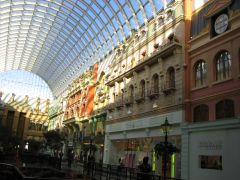
\includegraphics[width=.45\linewidth]{gfx/example_1}} \quad
        \subfloat[Pan ma signo.]
        {\label{fig:example-b}%
         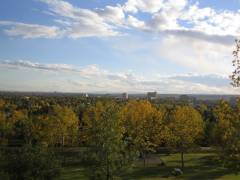
\includegraphics[width=.45\linewidth]{gfx/example_2}} \\
        \subfloat[Methodicamente o uno.]
        {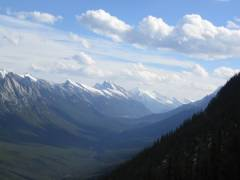
\includegraphics[width=.45\linewidth]{gfx/example_3}} \quad
        \subfloat[Titulo debitas.]
        {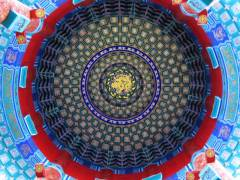
\includegraphics[width=.45\linewidth]{gfx/example_4}}
        \caption[Tu duo titulo debitas latente]{Tu duo titulo debitas
        latente. \ac{DRY}}\label{fig:example}
\end{figure}


%*****************************************
%*****************************************
%*****************************************
%*****************************************
%*****************************************

%%% Local Variables:
%%% mode: latex
%%% TeX-master: "../ClassicThesis"
%%% End:

%\addtocontents{toc}{\protect\clearpage} % <--- just debug stuff, ignore
%%************************************************
\chapter{Math Test Chapter}\label{ch:mathtest} % $\mathbb{ZNR}$
%************************************************
Ei choro aeterno antiopam mea, labitur bonorum pri no. His no decore
nemore graecis. In eos meis nominavi, liber soluta vim cu. Sea commune
suavitate interpretaris eu, vix eu libris efficiantur.

\section{Some Formulas}
Due to the statistical nature of ionisation energy loss, large
fluctuations can occur in the amount of energy deposited by a particle
traversing an absorber element\footnote{Examples taken from Walter
Schmidt's great gallery: \\
\url{http://home.vrweb.de/~was/mathfonts.html}}.  Continuous processes
such as multiple
scattering and energy loss play a relevant role in the longitudinal
and lateral development of electromagnetic and hadronic
showers, and in the case of sampling calorimeters the
measured resolution can be significantly affected by such fluctuations
in their active layers.  The description of ionisation fluctuations is
characterised by the significance parameter $\kappa$, which is
proportional to the ratio of mean energy loss to the maximum allowed
energy transfer in a single collision with an atomic electron:
\graffito{You might get unexpected results using math in chapter or
section heads. Consider the \texttt{pdfspacing} option.}
\begin{equation}
\kappa =\frac{\xi}{E_{\textrm{max}}} %\mathbb{ZNR}
\end{equation}
$E_{\textrm{max}}$ is the maximum transferable energy in a single
collision with an atomic electron.
\[
E_{\textrm{max}} =\frac{2 m_{\textrm{e}} \beta^2\gamma^2 }{1 +
2\gamma m_{\textrm{e}}/m_{\textrm{x}} + \left ( m_{\textrm{e}}
/m_{\textrm{x}}\right)^2}\ ,
\]
where $\gamma = E/m_{\textrm{x}}$, $E$ is energy and
$m_{\textrm{x}}$ the mass of the incident particle,
$\beta^2 = 1 - 1/\gamma^2$ and $m_{\textrm{e}}$ is the electron mass.
$\xi$ comes from the Rutherford scattering cross section
and is defined as:
\begin{eqnarray*} \xi  = \frac{2\pi z^2 e^4 N_{\textrm{Av}} Z \rho
\delta x}{m_{\textrm{e}} \beta^2 c^2 A} =  153.4 \frac{z^2}{\beta^2}
\frac{Z}{A}
  \rho \delta x \quad\textrm{keV},
\end{eqnarray*}
where

\begin{tabular}{ll}
$z$          & charge of the incident particle \\
$N_{\textrm{Av}}$     & Avogadro's number \\
$Z$          & atomic number of the material \\
$A$          & atomic weight of the material \\
$\rho$       & density \\
$ \delta x$  & thickness of the material \\
\end{tabular}

$\kappa$ measures the contribution of the collisions with energy
transfer close to $E_{\textrm{max}}$.  For a given absorber, $\kappa$
tends
towards large values if $\delta x$ is large and/or if $\beta$ is
small.  Likewise, $\kappa$ tends towards zero if $\delta x $ is small
and/or if $\beta$ approaches $1$.

The value of $\kappa$ distinguishes two regimes which occur in the
description of ionisation fluctuations:

\begin{enumerate}
\item A large number of collisions involving the loss of all or most
  of the incident particle energy during the traversal of an absorber.

  As the total energy transfer is composed of a multitude of small
  energy losses, we can apply the central limit theorem and describe
  the fluctuations by a Gaussian distribution.  This case is
  applicable to non-relativistic particles and is described by the
  inequality $\kappa > 10 $ (\ie, when the mean energy loss in the
  absorber is greater than the maximum energy transfer in a single
  collision).

\item Particles traversing thin counters and incident electrons under
  any conditions.

  The relevant inequalities and distributions are $ 0.01 < \kappa < 10
  $,
  Vavilov distribution, and $\kappa < 0.01 $, Landau distribution.
\end{enumerate}


\section{Various Mathematical Examples}
If $n > 2$, the identity
\[
  t[u_1,\dots,u_n] = t\bigl[t[u_1,\dots,u_{n_1}], t[u_2,\dots,u_n]
  \bigr]
\]
defines $t[u_1,\dots,u_n]$ recursively, and it can be shown that the
alternative definition
\[
  t[u_1,\dots,u_n] = t\bigl[t[u_1,u_2],\dots,t[u_{n-1},u_n]\bigr]
\]
gives the same result.  

%*****************************************
%*****************************************
%*****************************************
%*****************************************
%*****************************************

%%% Local Variables:
%%% mode: latex
%%% TeX-master: "../ClassicThesis"
%%% End:




%\include{multiToC} % <--- just debug stuff, ignore for your documents
% ********************************************************************
% Backmatter
%*******************************************************
\appendix
%\renewcommand{\thechapter}{\alph{chapter}}
\cleardoublepage
\part{Appendix}
%%********************************************************************
% Appendix
%*******************************************************
% If problems with the headers: get headings in appendix etc. right
%\markboth{\spacedlowsmallcaps{Appendix}}{\spacedlowsmallcaps{Appendix}}
\chapter{Appendix Test}
Lorem ipsum at nusquam appellantur his, ut eos erant homero
concludaturque. Albucius appellantur deterruisset id eam, vivendum
partiendo dissentiet ei ius. Vis melius facilisis ea, sea id convenire
referrentur, takimata adolescens ex duo. Ei harum argumentum per. Eam
vidit exerci appetere ad, ut vel zzril intellegam interpretaris.
\graffito{More dummy text.}

%Errem omnium ea per, pro congue populo ornatus cu, ex qui dicant
%nemore melius. No pri diam iriure euismod. Graecis eleifend
%appellantur quo id. Id corpora inimicus nam, facer nonummy ne pro,
%kasd repudiandae ei mei. Mea menandri mediocrem dissentiet cu, ex
%nominati imperdiet nec, sea odio duis vocent ei. Tempor everti
%appareat cu ius, ridens audiam an qui, aliquid admodum conceptam ne
%qui. Vis ea melius nostrum, mel alienum euripidis eu.

\section{Appendix Section Test}
Test: \autoref{tab:moreexample} (This reference should have a 
lowercase, small caps \spacedlowsmallcaps{A} if the option 
\texttt{floatperchapter} is activated, just as in the table itself
 $\rightarrow$ however, this does not work at the moment.)

\begin{table}[h]
    \myfloatalign
  \begin{tabularx}{\textwidth}{Xll} \toprule
    \tableheadline{labitur bonorum pri no} & \tableheadline{que vista}
    & \tableheadline{human} \\ \midrule
    fastidii ea ius & germano &  demonstratea \\
    suscipit instructior & titulo & personas \\
    %postulant quo & westeuropee & sanctificatec \\
    \midrule
    quaestio philosophia & facto & demonstrated \\
    %autem vulputate ex & parola & romanic \\
    %usu mucius iisque & studio & sanctificatef \\
    \bottomrule
  \end{tabularx}
  \caption[Autem usu id]{Autem usu id.}
  \label{tab:moreexample}
\end{table}

%Nulla fastidii ea ius, exerci suscipit instructior te nam, in ullum
%postulant quo. Congue quaestio philosophia his at, sea odio autem
%vulputate ex. Cu usu mucius iisque voluptua. Sit maiorum propriae at,
%ea cum primis intellegat. Hinc cotidieque reprehendunt eu nec. Autem
%timeam deleniti usu id, in nec nibh altera.




\section{Another Appendix Section Test}
Equidem detraxit cu nam, vix eu delenit periculis. Eos ut vero
constituto, no vidit propriae complectitur sea. Diceret nonummy in
has, no qui eligendi recteque consetetur. Mel eu dictas suscipiantur,
et sed placerat oporteat. At ipsum electram mei, ad aeque atomorum
mea. There is also a useless Pascal listing below: \autoref{lst:useless}.

\begin{lstlisting}[float=b,language=Pascal,frame=tb,caption={A floating example (\texttt{listings} manual)},label=lst:useless]
for i:=maxint downto 0 do
begin
{ do nothing }
end;
\end{lstlisting}

%Ei solet nemore consectetuer nam. Ad eam porro impetus, te choro omnes
%evertitur mel. Molestie conclusionemque vel at, no qui omittam
%expetenda efficiendi. Eu quo nobis offendit, verterem scriptorem ne
%vix.


%%% Local Variables:
%%% mode: latex
%%% TeX-master: "../ClassicThesis"
%%% End:

%********************************************************************
% Other Stuff in the Back
%*******************************************************
\cleardoublepage%********************************************************************
% Bibliography
%*******************************************************
% work-around to have small caps also here in the headline
\manualmark
\markboth{\spacedlowsmallcaps{\bibname}}{\spacedlowsmallcaps{\bibname}} % work-around to have small caps also
%\phantomsection 
\refstepcounter{dummy}
\addtocontents{toc}{\protect\vspace{\beforebibskip}} % to have the bib a bit from the rest in the toc
\addcontentsline{toc}{chapter}{\tocEntry{\bibname}}
\label{app:bibliography}
\printbibliography

%\cleardoublepage%*******************************************************
% Declaration
%*******************************************************
\refstepcounter{dummy}
\pdfbookmark[0]{Declaration}{declaration}
\chapter*{Declaration}
\thispagestyle{empty}
Put your declaration here.
\bigskip
 
\noindent\textit{\myLocation, \myTime}

\smallskip

\begin{flushright}
    \begin{tabular}{m{5cm}}
        \\ \hline
        \centering\myName \\
    \end{tabular}
\end{flushright}

%\cleardoublepage\pagestyle{empty}

\hfill

\vfill


\pdfbookmark[0]{Colophon}{colophon}
\section*{Colophon}
This document was typeset using the typographical look-and-feel \texttt{classicthesis} developed by Andr\'e Miede. 
The style was inspired by Robert Bringhurst's seminal book on typography ``\emph{The Elements of Typographic Style}''. 
\texttt{classicthesis} is available for both \LaTeX\ and \mLyX: 
\begin{center}
\url{https://bitbucket.org/amiede/classicthesis/}
\end{center}
Happy users of \texttt{classicthesis} usually send a real postcard to the author, a collection of postcards received so far is featured here: 
\begin{center}
\url{http://postcards.miede.de/}
\end{center}
 
\bigskip

\noindent\finalVersionString

%Hermann Zapf's \emph{Palatino} and \emph{Euler} type faces (Type~1 PostScript fonts \emph{URW
%Palladio L} and \emph{FPL}) are used. The ``typewriter'' text is typeset in \emph{Bera Mono}, 
%originally developed by Bitstream, Inc. as ``Bitstream Vera''. (Type~1 PostScript fonts were made 
%available by Malte Rosenau and
%Ulrich Dirr.)

%\paragraph{note:} The custom size of the textblock was calculated
%using the directions given by Mr. Bringhurst (pages 26--29 and
%175/176). 10~pt Palatino needs  133.21~pt for the string
%``abcdefghijklmnopqrstuvwxyz''. This yields a good line length between
%24--26~pc (288--312~pt). Using a ``\emph{double square textblock}''
%with a 1:2 ratio this results in a textblock of 312:624~pt (which
%includes the headline in this design). A good alternative would be the
%``\emph{golden section textblock}'' with a ratio of 1:1.62, here
%312:505.44~pt. For comparison, \texttt{DIV9} of the \texttt{typearea}
%package results in a line length of 389~pt (32.4~pc), which is by far
%too long. However, this information will only be of interest for
%hardcore pseudo-typographers like me.%
%
%To make your own calculations, use the following commands and look up
%the corresponding lengths in the book:
%\begin{verbatim}
%    \settowidth{\abcd}{abcdefghijklmnopqrstuvwxyz}
%    \the\abcd\ % prints the value of the length
%\end{verbatim}
%Please see the file \texttt{classicthesis.sty} for some precalculated 
%values for Palatino and Minion.
%
%    \settowidth{\abcd}{abcdefghijklmnopqrstuvwxyz}
%    \the\abcd\ % prints the value of the length





% ********************************************************************
% Game Over: Restore, Restart, or Quit?
%*******************************************************
\end{document}
% ********************************************************************

%%% Local Variables:
%%% mode: latex
%%% TeX-master: t
%%% End:
